\documentclass{article}
%%%%%%%%%%%%%%%%%%%%%%%%%%%%%%%%%%%%%%%%%%%%%%%%%%%%%%%%%%%%%%%%%%%%%%%%%%%%%%%%%%%%%%%%%%%%%%%%%%%%%%%%%%%%%%%%%%%%%%%%%%%%%%%%%%%%%%%%%%%%%%%%%%%%%%%%%%%%%%%%%%%%%%%%%%%%%%%%%%%%%%%%%%%%%%%%%%%%%%%%%%%%%%%%%%%%%%%%%%%%%%%%%%%%%%%%%%%%%%%%%%%%%%%%%%%%
\usepackage{amsmath}
\usepackage{amsfonts}
\usepackage{eurosym}
\usepackage[shortlabels]{enumitem}

\setcounter{MaxMatrixCols}{10}
%TCIDATA{OutputFilter=Latex.dll}
%TCIDATA{Version=5.50.0.2953}
%TCIDATA{<META NAME="SaveForMode" CONTENT="1">}
%TCIDATA{BibliographyScheme=Manual}
%TCIDATA{LastRevised=Friday, November 03, 2023 09:21:22}
%TCIDATA{<META NAME="GraphicsSave" CONTENT="32">}

\usepackage{graphicx}
\usepackage{subfig}

\DeclareMathOperator{\tr}{tr}
\DeclareMathOperator{\Tr}{Tr}

% Macros for Scientific Word and Scientific WorkPlace 5.5 documents saved with the LaTeX filter.
% Copyright (C) 2005 Mackichan Software, Inc.

\typeout{TCILATEX Macros for Scientific Word and Scientific WorkPlace 5.5 <06 Oct 2005>.}
\typeout{NOTICE:  This macro file is NOT proprietary and may be 
freely copied and distributed.}
%
\makeatletter

%%%%%%%%%%%%%%%%%%%%%
% pdfTeX related.
\ifx\pdfoutput\relax\let\pdfoutput=\undefined\fi
\newcount\msipdfoutput
\ifx\pdfoutput\undefined
\else
 \ifcase\pdfoutput
 \else 
    \msipdfoutput=1
    \ifx\paperwidth\undefined
    \else
      \ifdim\paperheight=0pt\relax
      \else
        \pdfpageheight\paperheight
      \fi
      \ifdim\paperwidth=0pt\relax
      \else
        \pdfpagewidth\paperwidth
      \fi
    \fi
  \fi  
\fi

%%%%%%%%%%%%%%%%%%%%%
% FMTeXButton
% This is used for putting TeXButtons in the 
% frontmatter of a document. Add a line like
% \QTagDef{FMTeXButton}{101}{} to the filter 
% section of the cst being used. Also add a
% new section containing:
%     [f_101]
%     ALIAS=FMTexButton
%     TAG_TYPE=FIELD
%     TAG_LEADIN=TeX Button:
%
% It also works to put \defs in the preamble after 
% the \input tcilatex
\def\FMTeXButton#1{#1}
%
%%%%%%%%%%%%%%%%%%%%%%
% macros for time
\newcount\@hour\newcount\@minute\chardef\@x10\chardef\@xv60
\def\tcitime{
\def\@time{%
  \@minute\time\@hour\@minute\divide\@hour\@xv
  \ifnum\@hour<\@x 0\fi\the\@hour:%
  \multiply\@hour\@xv\advance\@minute-\@hour
  \ifnum\@minute<\@x 0\fi\the\@minute
  }}%

%%%%%%%%%%%%%%%%%%%%%%
% macro for hyperref and msihyperref
%\@ifundefined{hyperref}{\def\hyperref#1#2#3#4{#2\ref{#4}#3}}{}

\def\x@hyperref#1#2#3{%
   % Turn off various catcodes before reading parameter 4
   \catcode`\~ = 12
   \catcode`\$ = 12
   \catcode`\_ = 12
   \catcode`\# = 12
   \catcode`\& = 12
   \catcode`\% = 12
   \y@hyperref{#1}{#2}{#3}%
}

\def\y@hyperref#1#2#3#4{%
   #2\ref{#4}#3
   \catcode`\~ = 13
   \catcode`\$ = 3
   \catcode`\_ = 8
   \catcode`\# = 6
   \catcode`\& = 4
   \catcode`\% = 14
}

\@ifundefined{hyperref}{\let\hyperref\x@hyperref}{}
\@ifundefined{msihyperref}{\let\msihyperref\x@hyperref}{}




% macro for external program call
\@ifundefined{qExtProgCall}{\def\qExtProgCall#1#2#3#4#5#6{\relax}}{}
%%%%%%%%%%%%%%%%%%%%%%
%
% macros for graphics
%
\def\FILENAME#1{#1}%
%
\def\QCTOpt[#1]#2{%
  \def\QCTOptB{#1}
  \def\QCTOptA{#2}
}
\def\QCTNOpt#1{%
  \def\QCTOptA{#1}
  \let\QCTOptB\empty
}
\def\Qct{%
  \@ifnextchar[{%
    \QCTOpt}{\QCTNOpt}
}
\def\QCBOpt[#1]#2{%
  \def\QCBOptB{#1}%
  \def\QCBOptA{#2}%
}
\def\QCBNOpt#1{%
  \def\QCBOptA{#1}%
  \let\QCBOptB\empty
}
\def\Qcb{%
  \@ifnextchar[{%
    \QCBOpt}{\QCBNOpt}%
}
\def\PrepCapArgs{%
  \ifx\QCBOptA\empty
    \ifx\QCTOptA\empty
      {}%
    \else
      \ifx\QCTOptB\empty
        {\QCTOptA}%
      \else
        [\QCTOptB]{\QCTOptA}%
      \fi
    \fi
  \else
    \ifx\QCBOptA\empty
      {}%
    \else
      \ifx\QCBOptB\empty
        {\QCBOptA}%
      \else
        [\QCBOptB]{\QCBOptA}%
      \fi
    \fi
  \fi
}
\newcount\GRAPHICSTYPE
%\GRAPHICSTYPE 0 is for TurboTeX
%\GRAPHICSTYPE 1 is for DVIWindo (PostScript)
%%%(removed)%\GRAPHICSTYPE 2 is for psfig (PostScript)
\GRAPHICSTYPE=\z@
\def\GRAPHICSPS#1{%
 \ifcase\GRAPHICSTYPE%\GRAPHICSTYPE=0
   \special{ps: #1}%
 \or%\GRAPHICSTYPE=1
   \special{language "PS", include "#1"}%
%%%\or%\GRAPHICSTYPE=2
%%%  #1%
 \fi
}%
%
\def\GRAPHICSHP#1{\special{include #1}}%
%
% \graffile{ body }                                  %#1
%          { contentswidth (scalar)  }               %#2
%          { contentsheight (scalar) }               %#3
%          { vertical shift when in-line (scalar) }  %#4

\def\graffile#1#2#3#4{%
%%% \ifnum\GRAPHICSTYPE=\tw@
%%%  %Following if using psfig
%%%  \@ifundefined{psfig}{\input psfig.tex}{}%
%%%  \psfig{file=#1, height=#3, width=#2}%
%%% \else
  %Following for all others
  % JCS - added BOXTHEFRAME, see below
    \bgroup
	   \@inlabelfalse
       \leavevmode
       \@ifundefined{bbl@deactivate}{\def~{\string~}}{\activesoff}%
        \raise -#4 \BOXTHEFRAME{%
           \hbox to #2{\raise #3\hbox to #2{\null #1\hfil}}}%
    \egroup
}%
%
% A box for drafts
\def\draftbox#1#2#3#4{%
 \leavevmode\raise -#4 \hbox{%
  \frame{\rlap{\protect\tiny #1}\hbox to #2%
   {\vrule height#3 width\z@ depth\z@\hfil}%
  }%
 }%
}%
%
\newcount\@msidraft
\@msidraft=\z@
\let\nographics=\@msidraft
\newif\ifwasdraft
\wasdraftfalse

%  \GRAPHIC{ body }                                  %#1
%          { draft name }                            %#2
%          { contentswidth (scalar)  }               %#3
%          { contentsheight (scalar) }               %#4
%          { vertical shift when in-line (scalar) }  %#5
\def\GRAPHIC#1#2#3#4#5{%
   \ifnum\@msidraft=\@ne\draftbox{#2}{#3}{#4}{#5}%
   \else\graffile{#1}{#3}{#4}{#5}%
   \fi
}
%
\def\addtoLaTeXparams#1{%
    \edef\LaTeXparams{\LaTeXparams #1}}%
%
% JCS -  added a switch BoxFrame that can 
% be set by including X in the frame params.
% If set a box is drawn around the frame.

\newif\ifBoxFrame \BoxFramefalse
\newif\ifOverFrame \OverFramefalse
\newif\ifUnderFrame \UnderFramefalse

\def\BOXTHEFRAME#1{%
   \hbox{%
      \ifBoxFrame
         \frame{#1}%
      \else
         {#1}%
      \fi
   }%
}


\def\doFRAMEparams#1{\BoxFramefalse\OverFramefalse\UnderFramefalse\readFRAMEparams#1\end}%
\def\readFRAMEparams#1{%
 \ifx#1\end%
  \let\next=\relax
  \else
  \ifx#1i\dispkind=\z@\fi
  \ifx#1d\dispkind=\@ne\fi
  \ifx#1f\dispkind=\tw@\fi
  \ifx#1t\addtoLaTeXparams{t}\fi
  \ifx#1b\addtoLaTeXparams{b}\fi
  \ifx#1p\addtoLaTeXparams{p}\fi
  \ifx#1h\addtoLaTeXparams{h}\fi
  \ifx#1X\BoxFrametrue\fi
  \ifx#1O\OverFrametrue\fi
  \ifx#1U\UnderFrametrue\fi
  \ifx#1w
    \ifnum\@msidraft=1\wasdrafttrue\else\wasdraftfalse\fi
    \@msidraft=\@ne
  \fi
  \let\next=\readFRAMEparams
  \fi
 \next
 }%
%
%Macro for In-line graphics object
%   \IFRAME{ contentswidth (scalar)  }               %#1
%          { contentsheight (scalar) }               %#2
%          { vertical shift when in-line (scalar) }  %#3
%          { draft name }                            %#4
%          { body }                                  %#5
%          { caption}                                %#6


\def\IFRAME#1#2#3#4#5#6{%
      \bgroup
      \let\QCTOptA\empty
      \let\QCTOptB\empty
      \let\QCBOptA\empty
      \let\QCBOptB\empty
      #6%
      \parindent=0pt
      \leftskip=0pt
      \rightskip=0pt
      \setbox0=\hbox{\QCBOptA}%
      \@tempdima=#1\relax
      \ifOverFrame
          % Do this later
          \typeout{This is not implemented yet}%
          \show\HELP
      \else
         \ifdim\wd0>\@tempdima
            \advance\@tempdima by \@tempdima
            \ifdim\wd0 >\@tempdima
               \setbox1 =\vbox{%
                  \unskip\hbox to \@tempdima{\hfill\GRAPHIC{#5}{#4}{#1}{#2}{#3}\hfill}%
                  \unskip\hbox to \@tempdima{\parbox[b]{\@tempdima}{\QCBOptA}}%
               }%
               \wd1=\@tempdima
            \else
               \textwidth=\wd0
               \setbox1 =\vbox{%
                 \noindent\hbox to \wd0{\hfill\GRAPHIC{#5}{#4}{#1}{#2}{#3}\hfill}\\%
                 \noindent\hbox{\QCBOptA}%
               }%
               \wd1=\wd0
            \fi
         \else
            \ifdim\wd0>0pt
              \hsize=\@tempdima
              \setbox1=\vbox{%
                \unskip\GRAPHIC{#5}{#4}{#1}{#2}{0pt}%
                \break
                \unskip\hbox to \@tempdima{\hfill \QCBOptA\hfill}%
              }%
              \wd1=\@tempdima
           \else
              \hsize=\@tempdima
              \setbox1=\vbox{%
                \unskip\GRAPHIC{#5}{#4}{#1}{#2}{0pt}%
              }%
              \wd1=\@tempdima
           \fi
         \fi
         \@tempdimb=\ht1
         %\advance\@tempdimb by \dp1
         \advance\@tempdimb by -#2
         \advance\@tempdimb by #3
         \leavevmode
         \raise -\@tempdimb \hbox{\box1}%
      \fi
      \egroup%
}%
%
%Macro for Display graphics object
%   \DFRAME{ contentswidth (scalar)  }               %#1
%          { contentsheight (scalar) }               %#2
%          { draft label }                           %#3
%          { name }                                  %#4
%          { caption}                                %#5
\def\DFRAME#1#2#3#4#5{%
  \vspace\topsep
  \hfil\break
  \bgroup
     \leftskip\@flushglue
	 \rightskip\@flushglue
	 \parindent\z@
	 \parfillskip\z@skip
     \let\QCTOptA\empty
     \let\QCTOptB\empty
     \let\QCBOptA\empty
     \let\QCBOptB\empty
	 \vbox\bgroup
        \ifOverFrame 
           #5\QCTOptA\par
        \fi
        \GRAPHIC{#4}{#3}{#1}{#2}{\z@}%
        \ifUnderFrame 
           \break#5\QCBOptA
        \fi
	 \egroup
  \egroup
  \vspace\topsep
  \break
}%
%
%Macro for Floating graphic object
%   \FFRAME{ framedata f|i tbph x F|T }              %#1
%          { contentswidth (scalar)  }               %#2
%          { contentsheight (scalar) }               %#3
%          { caption }                               %#4
%          { label }                                 %#5
%          { draft name }                            %#6
%          { body }                                  %#7
\def\FFRAME#1#2#3#4#5#6#7{%
 %If float.sty loaded and float option is 'h', change to 'H'  (gp) 1998/09/05
  \@ifundefined{floatstyle}
    {%floatstyle undefined (and float.sty not present), no change
     \begin{figure}[#1]%
    }
    {%floatstyle DEFINED
	 \ifx#1h%Only the h parameter, change to H
      \begin{figure}[H]%
	 \else
      \begin{figure}[#1]%
	 \fi
	}
  \let\QCTOptA\empty
  \let\QCTOptB\empty
  \let\QCBOptA\empty
  \let\QCBOptB\empty
  \ifOverFrame
    #4
    \ifx\QCTOptA\empty
    \else
      \ifx\QCTOptB\empty
        \caption{\QCTOptA}%
      \else
        \caption[\QCTOptB]{\QCTOptA}%
      \fi
    \fi
    \ifUnderFrame\else
      \label{#5}%
    \fi
  \else
    \UnderFrametrue%
  \fi
  \begin{center}\GRAPHIC{#7}{#6}{#2}{#3}{\z@}\end{center}%
  \ifUnderFrame
    #4
    \ifx\QCBOptA\empty
      \caption{}%
    \else
      \ifx\QCBOptB\empty
        \caption{\QCBOptA}%
      \else
        \caption[\QCBOptB]{\QCBOptA}%
      \fi
    \fi
    \label{#5}%
  \fi
  \end{figure}%
 }%
%
%
%    \FRAME{ framedata f|i tbph x F|T }              %#1
%          { contentswidth (scalar)  }               %#2
%          { contentsheight (scalar) }               %#3
%          { vertical shift when in-line (scalar) }  %#4
%          { caption }                               %#5
%          { label }                                 %#6
%          { name }                                  %#7
%          { body }                                  %#8
%
%    framedata is a string which can contain the following
%    characters: idftbphxFT
%    Their meaning is as follows:
%             i, d or f : in-line, display, or floating
%             t,b,p,h   : LaTeX floating placement options
%             x         : fit contents box to contents
%             F or T    : Figure or Table. 
%                         Later this can expand
%                         to a more general float class.
%
%
\newcount\dispkind%

\def\makeactives{
  \catcode`\"=\active
  \catcode`\;=\active
  \catcode`\:=\active
  \catcode`\'=\active
  \catcode`\~=\active
}
\bgroup
   \makeactives
   \gdef\activesoff{%
      \def"{\string"}%
      \def;{\string;}%
      \def:{\string:}%
      \def'{\string'}%
      \def~{\string~}%
      %\bbl@deactivate{"}%
      %\bbl@deactivate{;}%
      %\bbl@deactivate{:}%
      %\bbl@deactivate{'}%
    }
\egroup

\def\FRAME#1#2#3#4#5#6#7#8{%
 \bgroup
 \ifnum\@msidraft=\@ne
   \wasdrafttrue
 \else
   \wasdraftfalse%
 \fi
 \def\LaTeXparams{}%
 \dispkind=\z@
 \def\LaTeXparams{}%
 \doFRAMEparams{#1}%
 \ifnum\dispkind=\z@\IFRAME{#2}{#3}{#4}{#7}{#8}{#5}\else
  \ifnum\dispkind=\@ne\DFRAME{#2}{#3}{#7}{#8}{#5}\else
   \ifnum\dispkind=\tw@
    \edef\@tempa{\noexpand\FFRAME{\LaTeXparams}}%
    \@tempa{#2}{#3}{#5}{#6}{#7}{#8}%
    \fi
   \fi
  \fi
  \ifwasdraft\@msidraft=1\else\@msidraft=0\fi{}%
  \egroup
 }%
%
% This macro added to let SW gobble a parameter that
% should not be passed on and expanded. 

\def\TEXUX#1{"texux"}

%
% Macros for text attributes:
%
\def\BF#1{{\bf {#1}}}%
\def\NEG#1{\leavevmode\hbox{\rlap{\thinspace/}{$#1$}}}%
%
%%%%%%%%%%%%%%%%%%%%%%%%%%%%%%%%%%%%%%%%%%%%%%%%%%%%%%%%%%%%%%%%%%%%%%%%
%
%
% macros for user - defined functions
\def\limfunc#1{\mathop{\rm #1}}%
\def\func#1{\mathop{\rm #1}\nolimits}%
% macro for unit names
\def\unit#1{\mathord{\thinspace\rm #1}}%

%
% miscellaneous 
\long\def\QQQ#1#2{%
     \long\expandafter\def\csname#1\endcsname{#2}}%
\@ifundefined{QTP}{\def\QTP#1{}}{}
\@ifundefined{QEXCLUDE}{\def\QEXCLUDE#1{}}{}
\@ifundefined{Qlb}{\def\Qlb#1{#1}}{}
\@ifundefined{Qlt}{\def\Qlt#1{#1}}{}
\def\QWE{}%
\long\def\QQA#1#2{}%
\def\QTR#1#2{{\csname#1\endcsname {#2}}}%
  %	Add aliases for the ulem package
  \let\QQQuline\uline
  \let\QQQsout\sout
  \let\QQQuuline\uuline
  \let\QQQuwave\uwave
  \let\QQQxout\xout
\long\def\TeXButton#1#2{#2}%
\long\def\QSubDoc#1#2{#2}%
\def\EXPAND#1[#2]#3{}%
\def\NOEXPAND#1[#2]#3{}%
\def\PROTECTED{}%
\def\LaTeXparent#1{}%
\def\ChildStyles#1{}%
\def\ChildDefaults#1{}%
\def\QTagDef#1#2#3{}%

% Constructs added with Scientific Notebook
\@ifundefined{correctchoice}{\def\correctchoice{\relax}}{}
\@ifundefined{HTML}{\def\HTML#1{\relax}}{}
\@ifundefined{TCIIcon}{\def\TCIIcon#1#2#3#4{\relax}}{}
\if@compatibility
  \typeout{Not defining UNICODE  U or CustomNote commands for LaTeX 2.09.}
\else
  \providecommand{\UNICODE}[2][]{\protect\rule{.1in}{.1in}}
  \providecommand{\U}[1]{\protect\rule{.1in}{.1in}}
  \providecommand{\CustomNote}[3][]{\marginpar{#3}}
\fi

\@ifundefined{lambdabar}{
      \def\lambdabar{\errmessage{You have used the lambdabar symbol. 
                      This is available for typesetting only in RevTeX styles.}}
   }{}

%
% Macros for style editor docs
\@ifundefined{StyleEditBeginDoc}{\def\StyleEditBeginDoc{\relax}}{}
%
% Macros for footnotes
\def\QQfnmark#1{\footnotemark}
\def\QQfntext#1#2{\addtocounter{footnote}{#1}\footnotetext{#2}}
%
% Macros for indexing.
%
\@ifundefined{TCIMAKEINDEX}{}{\makeindex}%
%
% Attempts to avoid problems with other styles
\@ifundefined{abstract}{%
 \def\abstract{%
  \if@twocolumn
   \section*{Abstract (Not appropriate in this style!)}%
   \else \small 
   \begin{center}{\bf Abstract\vspace{-.5em}\vspace{\z@}}\end{center}%
   \quotation 
   \fi
  }%
 }{%
 }%
\@ifundefined{endabstract}{\def\endabstract
  {\if@twocolumn\else\endquotation\fi}}{}%
\@ifundefined{maketitle}{\def\maketitle#1{}}{}%
\@ifundefined{affiliation}{\def\affiliation#1{}}{}%
\@ifundefined{proof}{\def\proof{\noindent{\bfseries Proof. }}}{}%
\@ifundefined{endproof}{\def\endproof{\mbox{\ \rule{.1in}{.1in}}}}{}%
\@ifundefined{newfield}{\def\newfield#1#2{}}{}%
\@ifundefined{chapter}{\def\chapter#1{\par(Chapter head:)#1\par }%
 \newcount\c@chapter}{}%
\@ifundefined{part}{\def\part#1{\par(Part head:)#1\par }}{}%
\@ifundefined{section}{\def\section#1{\par(Section head:)#1\par }}{}%
\@ifundefined{subsection}{\def\subsection#1%
 {\par(Subsection head:)#1\par }}{}%
\@ifundefined{subsubsection}{\def\subsubsection#1%
 {\par(Subsubsection head:)#1\par }}{}%
\@ifundefined{paragraph}{\def\paragraph#1%
 {\par(Subsubsubsection head:)#1\par }}{}%
\@ifundefined{subparagraph}{\def\subparagraph#1%
 {\par(Subsubsubsubsection head:)#1\par }}{}%
%%%%%%%%%%%%%%%%%%%%%%%%%%%%%%%%%%%%%%%%%%%%%%%%%%%%%%%%%%%%%%%%%%%%%%%%
% These symbols are not recognized by LaTeX
\@ifundefined{therefore}{\def\therefore{}}{}%
\@ifundefined{backepsilon}{\def\backepsilon{}}{}%
\@ifundefined{yen}{\def\yen{\hbox{\rm\rlap=Y}}}{}%
\@ifundefined{registered}{%
   \def\registered{\relax\ifmmode{}\r@gistered
                    \else$\m@th\r@gistered$\fi}%
 \def\r@gistered{^{\ooalign
  {\hfil\raise.07ex\hbox{$\scriptstyle\rm\text{R}$}\hfil\crcr
  \mathhexbox20D}}}}{}%
\@ifundefined{Eth}{\def\Eth{}}{}%
\@ifundefined{eth}{\def\eth{}}{}%
\@ifundefined{Thorn}{\def\Thorn{}}{}%
\@ifundefined{thorn}{\def\thorn{}}{}%
% A macro to allow any symbol that requires math to appear in text
\def\TEXTsymbol#1{\mbox{$#1$}}%
\@ifundefined{degree}{\def\degree{{}^{\circ}}}{}%
%
% macros for T3TeX files
\newdimen\theight
\@ifundefined{Column}{\def\Column{%
 \vadjust{\setbox\z@=\hbox{\scriptsize\quad\quad tcol}%
  \theight=\ht\z@\advance\theight by \dp\z@\advance\theight by \lineskip
  \kern -\theight \vbox to \theight{%
   \rightline{\rlap{\box\z@}}%
   \vss
   }%
  }%
 }}{}%
%
\@ifundefined{qed}{\def\qed{%
 \ifhmode\unskip\nobreak\fi\ifmmode\ifinner\else\hskip5\p@\fi\fi
 \hbox{\hskip5\p@\vrule width4\p@ height6\p@ depth1.5\p@\hskip\p@}%
 }}{}%
%
\@ifundefined{cents}{\def\cents{\hbox{\rm\rlap c/}}}{}%
\@ifundefined{tciLaplace}{\def\tciLaplace{\ensuremath{\mathcal{L}}}}{}%
\@ifundefined{tciFourier}{\def\tciFourier{\ensuremath{\mathcal{F}}}}{}%
\@ifundefined{textcurrency}{\def\textcurrency{\hbox{\rm\rlap xo}}}{}%
\@ifundefined{texteuro}{\def\texteuro{\hbox{\rm\rlap C=}}}{}%
\@ifundefined{euro}{\def\euro{\hbox{\rm\rlap C=}}}{}%
\@ifundefined{textfranc}{\def\textfranc{\hbox{\rm\rlap-F}}}{}%
\@ifundefined{textlira}{\def\textlira{\hbox{\rm\rlap L=}}}{}%
\@ifundefined{textpeseta}{\def\textpeseta{\hbox{\rm P\negthinspace s}}}{}%
%
\@ifundefined{miss}{\def\miss{\hbox{\vrule height2\p@ width 2\p@ depth\z@}}}{}%
%
\@ifundefined{vvert}{\def\vvert{\Vert}}{}%  %always translated to \left| or \right|
%
\@ifundefined{tcol}{\def\tcol#1{{\baselineskip=6\p@ \vcenter{#1}} \Column}}{}%
%
\@ifundefined{dB}{\def\dB{\hbox{{}}}}{}%        %dummy entry in column 
\@ifundefined{mB}{\def\mB#1{\hbox{$#1$}}}{}%   %column entry
\@ifundefined{nB}{\def\nB#1{\hbox{#1}}}{}%     %column entry (not math)
%
\@ifundefined{note}{\def\note{$^{\dag}}}{}%
%
\def\newfmtname{LaTeX2e}
% No longer load latexsym.  This is now handled by SWP, which uses amsfonts if necessary
%
\ifx\fmtname\newfmtname
  \DeclareOldFontCommand{\rm}{\normalfont\rmfamily}{\mathrm}
  \DeclareOldFontCommand{\sf}{\normalfont\sffamily}{\mathsf}
  \DeclareOldFontCommand{\tt}{\normalfont\ttfamily}{\mathtt}
  \DeclareOldFontCommand{\bf}{\normalfont\bfseries}{\mathbf}
  \DeclareOldFontCommand{\it}{\normalfont\itshape}{\mathit}
  \DeclareOldFontCommand{\sl}{\normalfont\slshape}{\@nomath\sl}
  \DeclareOldFontCommand{\sc}{\normalfont\scshape}{\@nomath\sc}
\fi

%
% Greek bold macros
% Redefine all of the math symbols 
% which might be bolded	 - there are 
% probably others to add to this list

\def\alpha{{\Greekmath 010B}}%
\def\beta{{\Greekmath 010C}}%
\def\gamma{{\Greekmath 010D}}%
\def\delta{{\Greekmath 010E}}%
\def\epsilon{{\Greekmath 010F}}%
\def\zeta{{\Greekmath 0110}}%
\def\eta{{\Greekmath 0111}}%
\def\theta{{\Greekmath 0112}}%
\def\iota{{\Greekmath 0113}}%
\def\kappa{{\Greekmath 0114}}%
\def\lambda{{\Greekmath 0115}}%
\def\mu{{\Greekmath 0116}}%
\def\nu{{\Greekmath 0117}}%
\def\xi{{\Greekmath 0118}}%
\def\pi{{\Greekmath 0119}}%
\def\rho{{\Greekmath 011A}}%
\def\sigma{{\Greekmath 011B}}%
\def\tau{{\Greekmath 011C}}%
\def\upsilon{{\Greekmath 011D}}%
\def\phi{{\Greekmath 011E}}%
\def\chi{{\Greekmath 011F}}%
\def\psi{{\Greekmath 0120}}%
\def\omega{{\Greekmath 0121}}%
\def\varepsilon{{\Greekmath 0122}}%
\def\vartheta{{\Greekmath 0123}}%
\def\varpi{{\Greekmath 0124}}%
\def\varrho{{\Greekmath 0125}}%
\def\varsigma{{\Greekmath 0126}}%
\def\varphi{{\Greekmath 0127}}%

\def\nabla{{\Greekmath 0272}}
\def\FindBoldGroup{%
   {\setbox0=\hbox{$\mathbf{x\global\edef\theboldgroup{\the\mathgroup}}$}}%
}

\def\Greekmath#1#2#3#4{%
    \if@compatibility
        \ifnum\mathgroup=\symbold
           \mathchoice{\mbox{\boldmath$\displaystyle\mathchar"#1#2#3#4$}}%
                      {\mbox{\boldmath$\textstyle\mathchar"#1#2#3#4$}}%
                      {\mbox{\boldmath$\scriptstyle\mathchar"#1#2#3#4$}}%
                      {\mbox{\boldmath$\scriptscriptstyle\mathchar"#1#2#3#4$}}%
        \else
           \mathchar"#1#2#3#4% 
        \fi 
    \else 
        \FindBoldGroup
        \ifnum\mathgroup=\theboldgroup % For 2e
           \mathchoice{\mbox{\boldmath$\displaystyle\mathchar"#1#2#3#4$}}%
                      {\mbox{\boldmath$\textstyle\mathchar"#1#2#3#4$}}%
                      {\mbox{\boldmath$\scriptstyle\mathchar"#1#2#3#4$}}%
                      {\mbox{\boldmath$\scriptscriptstyle\mathchar"#1#2#3#4$}}%
        \else
           \mathchar"#1#2#3#4% 
        \fi     	    
	  \fi}

\newif\ifGreekBold  \GreekBoldfalse
\let\SAVEPBF=\pbf
\def\pbf{\GreekBoldtrue\SAVEPBF}%
%

\@ifundefined{theorem}{\newtheorem{theorem}{Theorem}}{}
\@ifundefined{lemma}{\newtheorem{lemma}[theorem]{Lemma}}{}
\@ifundefined{corollary}{\newtheorem{corollary}[theorem]{Corollary}}{}
\@ifundefined{conjecture}{\newtheorem{conjecture}[theorem]{Conjecture}}{}
\@ifundefined{proposition}{\newtheorem{proposition}[theorem]{Proposition}}{}
\@ifundefined{axiom}{\newtheorem{axiom}{Axiom}}{}
\@ifundefined{remark}{\newtheorem{remark}{Remark}}{}
\@ifundefined{example}{\newtheorem{example}{Example}}{}
\@ifundefined{exercise}{\newtheorem{exercise}{Exercise}}{}
\@ifundefined{definition}{\newtheorem{definition}{Definition}}{}


\@ifundefined{mathletters}{%
  %\def\theequation{\arabic{equation}}
  \newcounter{equationnumber}  
  \def\mathletters{%
     \addtocounter{equation}{1}
     \edef\@currentlabel{\theequation}%
     \setcounter{equationnumber}{\c@equation}
     \setcounter{equation}{0}%
     \edef\theequation{\@currentlabel\noexpand\alph{equation}}%
  }
  \def\endmathletters{%
     \setcounter{equation}{\value{equationnumber}}%
  }
}{}

%Logos
\@ifundefined{BibTeX}{%
    \def\BibTeX{{\rm B\kern-.05em{\sc i\kern-.025em b}\kern-.08em
                 T\kern-.1667em\lower.7ex\hbox{E}\kern-.125emX}}}{}%
\@ifundefined{AmS}%
    {\def\AmS{{\protect\usefont{OMS}{cmsy}{m}{n}%
                A\kern-.1667em\lower.5ex\hbox{M}\kern-.125emS}}}{}%
\@ifundefined{AmSTeX}{\def\AmSTeX{\protect\AmS-\protect\TeX\@}}{}%
%

% This macro is a fix to eqnarray
\def\@@eqncr{\let\@tempa\relax
    \ifcase\@eqcnt \def\@tempa{& & &}\or \def\@tempa{& &}%
      \else \def\@tempa{&}\fi
     \@tempa
     \if@eqnsw
        \iftag@
           \@taggnum
        \else
           \@eqnnum\stepcounter{equation}%
        \fi
     \fi
     \global\tag@false
     \global\@eqnswtrue
     \global\@eqcnt\z@\cr}


\def\TCItag{\@ifnextchar*{\@TCItagstar}{\@TCItag}}
\def\@TCItag#1{%
    \global\tag@true
    \global\def\@taggnum{(#1)}%
    \global\def\@currentlabel{#1}}
\def\@TCItagstar*#1{%
    \global\tag@true
    \global\def\@taggnum{#1}%
    \global\def\@currentlabel{#1}}
%
%%%%%%%%%%%%%%%%%%%%%%%%%%%%%%%%%%%%%%%%%%%%%%%%%%%%%%%%%%%%%%%%%%%%%
%
\def\QATOP#1#2{{#1 \atop #2}}%
\def\QTATOP#1#2{{\textstyle {#1 \atop #2}}}%
\def\QDATOP#1#2{{\displaystyle {#1 \atop #2}}}%
\def\QABOVE#1#2#3{{#2 \above#1 #3}}%
\def\QTABOVE#1#2#3{{\textstyle {#2 \above#1 #3}}}%
\def\QDABOVE#1#2#3{{\displaystyle {#2 \above#1 #3}}}%
\def\QOVERD#1#2#3#4{{#3 \overwithdelims#1#2 #4}}%
\def\QTOVERD#1#2#3#4{{\textstyle {#3 \overwithdelims#1#2 #4}}}%
\def\QDOVERD#1#2#3#4{{\displaystyle {#3 \overwithdelims#1#2 #4}}}%
\def\QATOPD#1#2#3#4{{#3 \atopwithdelims#1#2 #4}}%
\def\QTATOPD#1#2#3#4{{\textstyle {#3 \atopwithdelims#1#2 #4}}}%
\def\QDATOPD#1#2#3#4{{\displaystyle {#3 \atopwithdelims#1#2 #4}}}%
\def\QABOVED#1#2#3#4#5{{#4 \abovewithdelims#1#2#3 #5}}%
\def\QTABOVED#1#2#3#4#5{{\textstyle 
   {#4 \abovewithdelims#1#2#3 #5}}}%
\def\QDABOVED#1#2#3#4#5{{\displaystyle 
   {#4 \abovewithdelims#1#2#3 #5}}}%
%
% Macros for text size operators:
%

\def\tint{\msi@int\textstyle\int}%
\def\tiint{\msi@int\textstyle\iint}%
\def\tiiint{\msi@int\textstyle\iiint}%
\def\tiiiint{\msi@int\textstyle\iiiint}%
\def\tidotsint{\msi@int\textstyle\idotsint}%
\def\toint{\msi@int\textstyle\oint}%


\def\tsum{\mathop{\textstyle \sum }}%
\def\tprod{\mathop{\textstyle \prod }}%
\def\tbigcap{\mathop{\textstyle \bigcap }}%
\def\tbigwedge{\mathop{\textstyle \bigwedge }}%
\def\tbigoplus{\mathop{\textstyle \bigoplus }}%
\def\tbigodot{\mathop{\textstyle \bigodot }}%
\def\tbigsqcup{\mathop{\textstyle \bigsqcup }}%
\def\tcoprod{\mathop{\textstyle \coprod }}%
\def\tbigcup{\mathop{\textstyle \bigcup }}%
\def\tbigvee{\mathop{\textstyle \bigvee }}%
\def\tbigotimes{\mathop{\textstyle \bigotimes }}%
\def\tbiguplus{\mathop{\textstyle \biguplus }}%
%
%
%Macros for display size operators:
%

\newtoks\temptoksa
\newtoks\temptoksb
\newtoks\temptoksc


\def\msi@int#1#2{%
 \def\@temp{{#1#2\the\temptoksc_{\the\temptoksa}^{\the\temptoksb}}}%   
 \futurelet\@nextcs
 \@int
}

\def\@int{%
   \ifx\@nextcs\limits
      \typeout{Found limits}%
      \temptoksc={\limits}%
	  \let\@next\@intgobble%
   \else\ifx\@nextcs\nolimits
      \typeout{Found nolimits}%
      \temptoksc={\nolimits}%
	  \let\@next\@intgobble%
   \else
      \typeout{Did not find limits or no limits}%
      \temptoksc={}%
      \let\@next\msi@limits%
   \fi\fi
   \@next   
}%

\def\@intgobble#1{%
   \typeout{arg is #1}%
   \msi@limits
}


\def\msi@limits{%
   \temptoksa={}%
   \temptoksb={}%
   \@ifnextchar_{\@limitsa}{\@limitsb}%
}

\def\@limitsa_#1{%
   \temptoksa={#1}%
   \@ifnextchar^{\@limitsc}{\@temp}%
}

\def\@limitsb{%
   \@ifnextchar^{\@limitsc}{\@temp}%
}

\def\@limitsc^#1{%
   \temptoksb={#1}%
   \@ifnextchar_{\@limitsd}{\@temp}%   
}

\def\@limitsd_#1{%
   \temptoksa={#1}%
   \@temp
}



\def\dint{\msi@int\displaystyle\int}%
\def\diint{\msi@int\displaystyle\iint}%
\def\diiint{\msi@int\displaystyle\iiint}%
\def\diiiint{\msi@int\displaystyle\iiiint}%
\def\didotsint{\msi@int\displaystyle\idotsint}%
\def\doint{\msi@int\displaystyle\oint}%

\def\dsum{\mathop{\displaystyle \sum }}%
\def\dprod{\mathop{\displaystyle \prod }}%
\def\dbigcap{\mathop{\displaystyle \bigcap }}%
\def\dbigwedge{\mathop{\displaystyle \bigwedge }}%
\def\dbigoplus{\mathop{\displaystyle \bigoplus }}%
\def\dbigodot{\mathop{\displaystyle \bigodot }}%
\def\dbigsqcup{\mathop{\displaystyle \bigsqcup }}%
\def\dcoprod{\mathop{\displaystyle \coprod }}%
\def\dbigcup{\mathop{\displaystyle \bigcup }}%
\def\dbigvee{\mathop{\displaystyle \bigvee }}%
\def\dbigotimes{\mathop{\displaystyle \bigotimes }}%
\def\dbiguplus{\mathop{\displaystyle \biguplus }}%

\if@compatibility\else
  % Always load amsmath in LaTeX2e mode
  \RequirePackage{amsmath}
\fi

\def\ExitTCILatex{\makeatother\endinput}

\bgroup
\ifx\ds@amstex\relax
   \message{amstex already loaded}\aftergroup\ExitTCILatex
\else
   \@ifpackageloaded{amsmath}%
      {\if@compatibility\message{amsmath already loaded}\fi\aftergroup\ExitTCILatex}
      {}
   \@ifpackageloaded{amstex}%
      {\if@compatibility\message{amstex already loaded}\fi\aftergroup\ExitTCILatex}
      {}
   \@ifpackageloaded{amsgen}%
      {\if@compatibility\message{amsgen already loaded}\fi\aftergroup\ExitTCILatex}
      {}
\fi
\egroup

%Exit if any of the AMS macros are already loaded.
%This is always the case for LaTeX2e mode.


%%%%%%%%%%%%%%%%%%%%%%%%%%%%%%%%%%%%%%%%%%%%%%%%%%%%%%%%%%%%%%%%%%%%%%%%%%
% NOTE: The rest of this file is read only if in LaTeX 2.09 compatibility
% mode. This section is used to define AMS-like constructs in the
% event they have not been defined.
%%%%%%%%%%%%%%%%%%%%%%%%%%%%%%%%%%%%%%%%%%%%%%%%%%%%%%%%%%%%%%%%%%%%%%%%%%
\typeout{TCILATEX defining AMS-like constructs in LaTeX 2.09 COMPATIBILITY MODE}
%%%%%%%%%%%%%%%%%%%%%%%%%%%%%%%%%%%%%%%%%%%%%%%%%%%%%%%%%%%%%%%%%%%%%%%%
%  Macros to define some AMS LaTeX constructs when 
%  AMS LaTeX has not been loaded
% 
% These macros are copied from the AMS-TeX package for doing
% multiple integrals.
%
\let\DOTSI\relax
\def\RIfM@{\relax\ifmmode}%
\def\FN@{\futurelet\next}%
\newcount\intno@
\def\iint{\DOTSI\intno@\tw@\FN@\ints@}%
\def\iiint{\DOTSI\intno@\thr@@\FN@\ints@}%
\def\iiiint{\DOTSI\intno@4 \FN@\ints@}%
\def\idotsint{\DOTSI\intno@\z@\FN@\ints@}%
\def\ints@{\findlimits@\ints@@}%
\newif\iflimtoken@
\newif\iflimits@
\def\findlimits@{\limtoken@true\ifx\next\limits\limits@true
 \else\ifx\next\nolimits\limits@false\else
 \limtoken@false\ifx\ilimits@\nolimits\limits@false\else
 \ifinner\limits@false\else\limits@true\fi\fi\fi\fi}%
\def\multint@{\int\ifnum\intno@=\z@\intdots@                          %1
 \else\intkern@\fi                                                    %2
 \ifnum\intno@>\tw@\int\intkern@\fi                                   %3
 \ifnum\intno@>\thr@@\int\intkern@\fi                                 %4
 \int}%                                                               %5
\def\multintlimits@{\intop\ifnum\intno@=\z@\intdots@\else\intkern@\fi
 \ifnum\intno@>\tw@\intop\intkern@\fi
 \ifnum\intno@>\thr@@\intop\intkern@\fi\intop}%
\def\intic@{%
    \mathchoice{\hskip.5em}{\hskip.4em}{\hskip.4em}{\hskip.4em}}%
\def\negintic@{\mathchoice
 {\hskip-.5em}{\hskip-.4em}{\hskip-.4em}{\hskip-.4em}}%
\def\ints@@{\iflimtoken@                                              %1
 \def\ints@@@{\iflimits@\negintic@
   \mathop{\intic@\multintlimits@}\limits                             %2
  \else\multint@\nolimits\fi                                          %3
  \eat@}%                                                             %4
 \else                                                                %5
 \def\ints@@@{\iflimits@\negintic@
  \mathop{\intic@\multintlimits@}\limits\else
  \multint@\nolimits\fi}\fi\ints@@@}%
\def\intkern@{\mathchoice{\!\!\!}{\!\!}{\!\!}{\!\!}}%
\def\plaincdots@{\mathinner{\cdotp\cdotp\cdotp}}%
\def\intdots@{\mathchoice{\plaincdots@}%
 {{\cdotp}\mkern1.5mu{\cdotp}\mkern1.5mu{\cdotp}}%
 {{\cdotp}\mkern1mu{\cdotp}\mkern1mu{\cdotp}}%
 {{\cdotp}\mkern1mu{\cdotp}\mkern1mu{\cdotp}}}%
%
%
%  These macros are for doing the AMS \text{} construct
%
\def\RIfM@{\relax\protect\ifmmode}
\def\text{\RIfM@\expandafter\text@\else\expandafter\mbox\fi}
\let\nfss@text\text
\def\text@#1{\mathchoice
   {\textdef@\displaystyle\f@size{#1}}%
   {\textdef@\textstyle\tf@size{\firstchoice@false #1}}%
   {\textdef@\textstyle\sf@size{\firstchoice@false #1}}%
   {\textdef@\textstyle \ssf@size{\firstchoice@false #1}}%
   \glb@settings}

\def\textdef@#1#2#3{\hbox{{%
                    \everymath{#1}%
                    \let\f@size#2\selectfont
                    #3}}}
\newif\iffirstchoice@
\firstchoice@true
%
%These are the AMS constructs for multiline limits.
%
\def\Let@{\relax\iffalse{\fi\let\\=\cr\iffalse}\fi}%
\def\vspace@{\def\vspace##1{\crcr\noalign{\vskip##1\relax}}}%
\def\multilimits@{\bgroup\vspace@\Let@
 \baselineskip\fontdimen10 \scriptfont\tw@
 \advance\baselineskip\fontdimen12 \scriptfont\tw@
 \lineskip\thr@@\fontdimen8 \scriptfont\thr@@
 \lineskiplimit\lineskip
 \vbox\bgroup\ialign\bgroup\hfil$\m@th\scriptstyle{##}$\hfil\crcr}%
\def\Sb{_\multilimits@}%
\def\endSb{\crcr\egroup\egroup\egroup}%
\def\Sp{^\multilimits@}%
\let\endSp\endSb
%
%
%These are AMS constructs for horizontal arrows
%
\newdimen\ex@
\ex@.2326ex
\def\rightarrowfill@#1{$#1\m@th\mathord-\mkern-6mu\cleaders
 \hbox{$#1\mkern-2mu\mathord-\mkern-2mu$}\hfill
 \mkern-6mu\mathord\rightarrow$}%
\def\leftarrowfill@#1{$#1\m@th\mathord\leftarrow\mkern-6mu\cleaders
 \hbox{$#1\mkern-2mu\mathord-\mkern-2mu$}\hfill\mkern-6mu\mathord-$}%
\def\leftrightarrowfill@#1{$#1\m@th\mathord\leftarrow
\mkern-6mu\cleaders
 \hbox{$#1\mkern-2mu\mathord-\mkern-2mu$}\hfill
 \mkern-6mu\mathord\rightarrow$}%
\def\overrightarrow{\mathpalette\overrightarrow@}%
\def\overrightarrow@#1#2{\vbox{\ialign{##\crcr\rightarrowfill@#1\crcr
 \noalign{\kern-\ex@\nointerlineskip}$\m@th\hfil#1#2\hfil$\crcr}}}%
\let\overarrow\overrightarrow
\def\overleftarrow{\mathpalette\overleftarrow@}%
\def\overleftarrow@#1#2{\vbox{\ialign{##\crcr\leftarrowfill@#1\crcr
 \noalign{\kern-\ex@\nointerlineskip}$\m@th\hfil#1#2\hfil$\crcr}}}%
\def\overleftrightarrow{\mathpalette\overleftrightarrow@}%
\def\overleftrightarrow@#1#2{\vbox{\ialign{##\crcr
   \leftrightarrowfill@#1\crcr
 \noalign{\kern-\ex@\nointerlineskip}$\m@th\hfil#1#2\hfil$\crcr}}}%
\def\underrightarrow{\mathpalette\underrightarrow@}%
\def\underrightarrow@#1#2{\vtop{\ialign{##\crcr$\m@th\hfil#1#2\hfil
  $\crcr\noalign{\nointerlineskip}\rightarrowfill@#1\crcr}}}%
\let\underarrow\underrightarrow
\def\underleftarrow{\mathpalette\underleftarrow@}%
\def\underleftarrow@#1#2{\vtop{\ialign{##\crcr$\m@th\hfil#1#2\hfil
  $\crcr\noalign{\nointerlineskip}\leftarrowfill@#1\crcr}}}%
\def\underleftrightarrow{\mathpalette\underleftrightarrow@}%
\def\underleftrightarrow@#1#2{\vtop{\ialign{##\crcr$\m@th
  \hfil#1#2\hfil$\crcr
 \noalign{\nointerlineskip}\leftrightarrowfill@#1\crcr}}}%
%%%%%%%%%%%%%%%%%%%%%

\def\qopnamewl@#1{\mathop{\operator@font#1}\nlimits@}
\let\nlimits@\displaylimits
\def\setboxz@h{\setbox\z@\hbox}


\def\varlim@#1#2{\mathop{\vtop{\ialign{##\crcr
 \hfil$#1\m@th\operator@font lim$\hfil\crcr
 \noalign{\nointerlineskip}#2#1\crcr
 \noalign{\nointerlineskip\kern-\ex@}\crcr}}}}

 \def\rightarrowfill@#1{\m@th\setboxz@h{$#1-$}\ht\z@\z@
  $#1\copy\z@\mkern-6mu\cleaders
  \hbox{$#1\mkern-2mu\box\z@\mkern-2mu$}\hfill
  \mkern-6mu\mathord\rightarrow$}
\def\leftarrowfill@#1{\m@th\setboxz@h{$#1-$}\ht\z@\z@
  $#1\mathord\leftarrow\mkern-6mu\cleaders
  \hbox{$#1\mkern-2mu\copy\z@\mkern-2mu$}\hfill
  \mkern-6mu\box\z@$}


\def\projlim{\qopnamewl@{proj\,lim}}
\def\injlim{\qopnamewl@{inj\,lim}}
\def\varinjlim{\mathpalette\varlim@\rightarrowfill@}
\def\varprojlim{\mathpalette\varlim@\leftarrowfill@}
\def\varliminf{\mathpalette\varliminf@{}}
\def\varliminf@#1{\mathop{\underline{\vrule\@depth.2\ex@\@width\z@
   \hbox{$#1\m@th\operator@font lim$}}}}
\def\varlimsup{\mathpalette\varlimsup@{}}
\def\varlimsup@#1{\mathop{\overline
  {\hbox{$#1\m@th\operator@font lim$}}}}

%
%Companion to stackrel
\def\stackunder#1#2{\mathrel{\mathop{#2}\limits_{#1}}}%
%
%
% These are AMS environments that will be defined to
% be verbatims if amstex has not actually been 
% loaded
%
%
\begingroup \catcode `|=0 \catcode `[= 1
\catcode`]=2 \catcode `\{=12 \catcode `\}=12
\catcode`\\=12 
|gdef|@alignverbatim#1\end{align}[#1|end[align]]
|gdef|@salignverbatim#1\end{align*}[#1|end[align*]]

|gdef|@alignatverbatim#1\end{alignat}[#1|end[alignat]]
|gdef|@salignatverbatim#1\end{alignat*}[#1|end[alignat*]]

|gdef|@xalignatverbatim#1\end{xalignat}[#1|end[xalignat]]
|gdef|@sxalignatverbatim#1\end{xalignat*}[#1|end[xalignat*]]

|gdef|@gatherverbatim#1\end{gather}[#1|end[gather]]
|gdef|@sgatherverbatim#1\end{gather*}[#1|end[gather*]]

|gdef|@gatherverbatim#1\end{gather}[#1|end[gather]]
|gdef|@sgatherverbatim#1\end{gather*}[#1|end[gather*]]


|gdef|@multilineverbatim#1\end{multiline}[#1|end[multiline]]
|gdef|@smultilineverbatim#1\end{multiline*}[#1|end[multiline*]]

|gdef|@arraxverbatim#1\end{arrax}[#1|end[arrax]]
|gdef|@sarraxverbatim#1\end{arrax*}[#1|end[arrax*]]

|gdef|@tabulaxverbatim#1\end{tabulax}[#1|end[tabulax]]
|gdef|@stabulaxverbatim#1\end{tabulax*}[#1|end[tabulax*]]


|endgroup
  

  
\def\align{\@verbatim \frenchspacing\@vobeyspaces \@alignverbatim
You are using the "align" environment in a style in which it is not defined.}
\let\endalign=\endtrivlist
 
\@namedef{align*}{\@verbatim\@salignverbatim
You are using the "align*" environment in a style in which it is not defined.}
\expandafter\let\csname endalign*\endcsname =\endtrivlist




\def\alignat{\@verbatim \frenchspacing\@vobeyspaces \@alignatverbatim
You are using the "alignat" environment in a style in which it is not defined.}
\let\endalignat=\endtrivlist
 
\@namedef{alignat*}{\@verbatim\@salignatverbatim
You are using the "alignat*" environment in a style in which it is not defined.}
\expandafter\let\csname endalignat*\endcsname =\endtrivlist




\def\xalignat{\@verbatim \frenchspacing\@vobeyspaces \@xalignatverbatim
You are using the "xalignat" environment in a style in which it is not defined.}
\let\endxalignat=\endtrivlist
 
\@namedef{xalignat*}{\@verbatim\@sxalignatverbatim
You are using the "xalignat*" environment in a style in which it is not defined.}
\expandafter\let\csname endxalignat*\endcsname =\endtrivlist




\def\gather{\@verbatim \frenchspacing\@vobeyspaces \@gatherverbatim
You are using the "gather" environment in a style in which it is not defined.}
\let\endgather=\endtrivlist
 
\@namedef{gather*}{\@verbatim\@sgatherverbatim
You are using the "gather*" environment in a style in which it is not defined.}
\expandafter\let\csname endgather*\endcsname =\endtrivlist


\def\multiline{\@verbatim \frenchspacing\@vobeyspaces \@multilineverbatim
You are using the "multiline" environment in a style in which it is not defined.}
\let\endmultiline=\endtrivlist
 
\@namedef{multiline*}{\@verbatim\@smultilineverbatim
You are using the "multiline*" environment in a style in which it is not defined.}
\expandafter\let\csname endmultiline*\endcsname =\endtrivlist


\def\arrax{\@verbatim \frenchspacing\@vobeyspaces \@arraxverbatim
You are using a type of "array" construct that is only allowed in AmS-LaTeX.}
\let\endarrax=\endtrivlist

\def\tabulax{\@verbatim \frenchspacing\@vobeyspaces \@tabulaxverbatim
You are using a type of "tabular" construct that is only allowed in AmS-LaTeX.}
\let\endtabulax=\endtrivlist

 
\@namedef{arrax*}{\@verbatim\@sarraxverbatim
You are using a type of "array*" construct that is only allowed in AmS-LaTeX.}
\expandafter\let\csname endarrax*\endcsname =\endtrivlist

\@namedef{tabulax*}{\@verbatim\@stabulaxverbatim
You are using a type of "tabular*" construct that is only allowed in AmS-LaTeX.}
\expandafter\let\csname endtabulax*\endcsname =\endtrivlist

% macro to simulate ams tag construct


% This macro is a fix to the equation environment
 \def\endequation{%
     \ifmmode\ifinner % FLEQN hack
      \iftag@
        \addtocounter{equation}{-1} % undo the increment made in the begin part
        $\hfil
           \displaywidth\linewidth\@taggnum\egroup \endtrivlist
        \global\tag@false
        \global\@ignoretrue   
      \else
        $\hfil
           \displaywidth\linewidth\@eqnnum\egroup \endtrivlist
        \global\tag@false
        \global\@ignoretrue 
      \fi
     \else   
      \iftag@
        \addtocounter{equation}{-1} % undo the increment made in the begin part
        \eqno \hbox{\@taggnum}
        \global\tag@false%
        $$\global\@ignoretrue
      \else
        \eqno \hbox{\@eqnnum}% $$ BRACE MATCHING HACK
        $$\global\@ignoretrue
      \fi
     \fi\fi
 } 

 \newif\iftag@ \tag@false
 
 \def\TCItag{\@ifnextchar*{\@TCItagstar}{\@TCItag}}
 \def\@TCItag#1{%
     \global\tag@true
     \global\def\@taggnum{(#1)}%
     \global\def\@currentlabel{#1}}
 \def\@TCItagstar*#1{%
     \global\tag@true
     \global\def\@taggnum{#1}%
     \global\def\@currentlabel{#1}}

  \@ifundefined{tag}{
     \def\tag{\@ifnextchar*{\@tagstar}{\@tag}}
     \def\@tag#1{%
         \global\tag@true
         \global\def\@taggnum{(#1)}}
     \def\@tagstar*#1{%
         \global\tag@true
         \global\def\@taggnum{#1}}
  }{}

\def\tfrac#1#2{{\textstyle {#1 \over #2}}}%
\def\dfrac#1#2{{\displaystyle {#1 \over #2}}}%
\def\binom#1#2{{#1 \choose #2}}%
\def\tbinom#1#2{{\textstyle {#1 \choose #2}}}%
\def\dbinom#1#2{{\displaystyle {#1 \choose #2}}}%

% Do not add anything to the end of this file.  
% The last section of the file is loaded only if 
% amstex has not been.
\makeatother
\endinput


\begin{document}

\title{Tomographic universality of the discrete Wigner function}

\begin{abstract}
We observe that the Discrete Wigner function (DWF) for $n$-partite systems with
odd local dimensions are tomographically universal, as reflected in a
delta-function form of the DWF for any stabilizer. However, in the $n$-qubit
case this property does not hold due to the non-factorization of the mapping
kernel, whose explicit form depends on a particular partition of the discrete
phase-space. Nonetheless, it turns out that the DWF for some specific
stabilizers, not included in the set used for the construction of the Wigner
map, takes on the form of a delta-function. This implies that the possibility of
classical simulations of Pauli measurements in a given stabilizer state for
qubit systems is closely tied to the experimental setup.
\end{abstract}

\author{
  Isabel Sainz$^{1}$ 0000-0002-6671-0262,
  Ernesto Camacho$^{2}$,
  Andrés García$^{2}$
  and Andrei B. Klimov$^{1}$ 0000-0001-8493-721X \\
  $^{1}$ \quad Departamento de Física, Universidad de Guadalajara, Revolución
  1500, 44420, Guadalajara, Jal., México\\
  $^{2}$ \quad Departamento de Matemáticas, Universidad de Guadalajara,
  Revolución 1500, 44420, Guadalajara, Jal., México\\
  \ddag\ These authors contributed equally to this work.
}

\maketitle

\section{Introduction}

The concept of quasidistribution functions, which emerged as a means to
incorporate quantum corrections into statistical mechanics within two
distinct contexts \cite{wigner,bloch}, has been successfully used to
reformulate quantum mechanics in position and momentum (plane) phase space 
\cite{groenewold,moyal}. Subsequently, these concepts were generalized to
more sophisticated geometries. In the framework of the phase-space approach,
operators suitable for a given quantum system are represented as real
functions obtained from an invertible and covariant linear map $\hat{w}%
(\Omega )$,%
\begin{equation*}
\hat{f}\Leftrightarrow W_{f}(\Omega )=Tr\left( \hat{f}\hat{w}(\Omega
)\right) ,\quad
\end{equation*}%
where $\Omega $ is a point in the corresponding phase-space $\mathcal{M}$.

The most natural and widely used representation
\cite{qoptics,electron1,electron2} commonly referred to as the Wigner
correspondence \cite{wigner} is self-dual. This self-duality allows for the
treatment of both states and observables in the same manner, making it
particularly useful for studying the quantum-classical correspondence \cite%
{berry}. However, the main drawback of the Wigner map lies in its
representation of some states in the form of negative (quasi)-distributions.
In fact, it's noteworthy that non-negative Wigner functions (WF) correspond
only to the so-called Gaussian states, thereby restricting the type of
positivity-preserving operations to Gaussian ones.

A discrete analogue of the Wigner map, which is applicable for describing a
finite number of particles with a local dimension that is a prime number,
was introduced significantly later \cite{spin1, spin2,wootters1,gibbons}.
This discrete analog has recently found remarkable applications in the
analysis of classicality and the (classical) simulability of $n$-partite
quantum systems \cite{gottKnill, galvao, cormick, gross,WignerNegResource,
Raus17, UniqueWF, cohomo}. In this context, the discrete phase-space (DPS) $%
\mathcal{M}$ takes the form of a $p^{n}\times p^{n}$ grid, constituting an
affine plane \cite{Saniga2004}. By labeling it with elements from the Galois
field $\mathbb{F}_{p^{n}}$ , this DPS inherits the same geometric properties as
the ordinary plane, e.g., parallel lines (not necessarily straight) do not
intersect, etc.

The construction of discrete quasidistributions is closely tied to the
concept of Mutually Unbiased Bases (MUBs) \cite{ivanovic,mubs1,mubs2}, which
are eigenstates of disjoint sets of $p^{n}$ commuting monomials
(stabilizers) formed by products of the generalized Pauli operators. In
power-of-prime dimensions one can always arrange the operational basis
formed by $p^{2n}-1$ monomials (excluding the identity operator) into $%
p^{n}+1$ disjoint stabilizers ~\cite{Bandyopadhyay2002}. In addition, it is
possible to associate lines in the DPS with projectors onto elements of a
certain (stabilizer) basis in a way that non-intersecting lines correspond
to mutually unbiased bases \cite{wootters1}. It is noteworthy that in the
prime-dimensional case only straight lines can be related to MUBs. However,
in power-of-prime dimensions such an association exists with more complex
geometrical structures, the so-called commutative curves \cite{GS2,JPA09}.
This leads to a fundamental property of the discrete Wigner function: the
tomographic condition. This condition means that summing the Wigner function
over a line results in the probability that the system is in the state
associated with that particular line \cite{wootters1, gibbons}.

The mapping kernel from the Hilbert space into the DPS can be recast as a sum of
projectors onto elements of an appropriate complete set of MUBs. However, there
are several inequivalent ways to form $p^{n}+1$ disjoint commuting sets,
which correspond to different partitions of the DPS into non-intersecting
curves. Such sets can be roughly characterized by their factorization
properties and both unitary equivalent and (globally) unitary inequivalent
sets of stabilizers can be found. Consequently, the form of the discrete
self-dual maps fundamentally depends on the chosen complete set of
stabilizers \cite{Bjork2007}. For each state of the MUBs used in the
construction of the mapping kernel, the Wigner function is represented as a
delta-function. The later is equivalent to the tomographic condition \cite%
{gibbons,galvao,cormick,DFW11,DFW12}.

On the other hand, it's known that the Wigner map for odd-prime local
dimensions exhibits a property akin to the continuous position-momentum
Wigner function: only stabilizer states correspond to non-negative Wigner
functions \cite{gross}. This characteristic arises from the factorization of
the self-dual mapping kernel for any partition of the DPS and results in
tomographic universality of the DWFs, which acquire a delta-function form
for any stabilizer state of any partition. It enables the use of the DWF as
an indicator of quantumness, allowing the classification of quantum states
based on their suitability for quantum computation speedup and estimation of
the cost of classically simulating quantum circuits \cite{Raus17,UniqueWF,
cohomo, contextMagic, WignerContext}.

However, this property breaks down in the case of qubit systems \cite{
UniqueWF, cohomo,contextMagic}. The main reason for the loss of tomographic
universality in $n$-qubit systems is the inequivalence among Wigner maps
based on different sets of stabilizers \cite{Bjork2007}, \cite{qip17}. This
leads to the following question: Is it possible for the DWF of an element of
a stabilizer basis to take on the form of a delta-function if that basis is
not used for the construction of the Wigner map? In other words, are there
states, aside from the elements of the MUBs fixing the map, that satisfy the
tomographic condition?

In this paper, we show that in the $n$-qubit case, when a partition of the
discrete phase-space into a complete fixed set of stabilizers is given, it
is possible to identify stabilizer states whose Wigner functions take on the
form of delta functions along commutative curves belonging to other
partitions. We analyze explicit results for the three-qubit case and discuss
the implications of this observed property of $n$-qubit DWFs.

\section{The generalized Pauli group and displacement operators}

Let us consider a system of $n$ qudits, each with a \textit{local} dimension
that is a prime number $p$. It is convenient to relabel vectors of an
orthonormal basis $|k_{1},\ldots ,k_{n}\rangle $ ($k_{i}\in \mathbb{Z}_{p}$) in
the corresponding Hilbert space $\mathcal{H}_{p^{n}}=\mathcal{H}_{p}^{\otimes
n}$ by elements of a finite field, $|\kappa \rangle $, $\kappa \in \mathbb{F}%
_{p^{n}}$ according to 
\begin{equation}
  |k_{1},\ldots ,k_{n}\rangle \Leftrightarrow |\kappa \rangle,
  \quad \langle
  \kappa^{\prime}|\kappa \rangle =\delta _{\kappa ^{\prime },\kappa },
  \quad
  \kappa =\sum_{i=1}^{n}k_{i}\,\theta _{i}\in \mathbb{F}_{p^{n}},
  \label{basis}
\end{equation}%
where $\{\theta_{1},\ldots ,\theta_{n}\}$ is an abstract basis in the
field $\mathbb{F}_{p^{n}}$, considered as a linear space; the components
$k_{i}$, $i=1,..,n$ are obtained through the trace operation with a dual basis,
$\{\tilde{\theta}_{1},\ldots ,\tilde{\theta}_{n}\}$ [i.e., $\tr(\theta
_{i}\,\tilde{\theta}_{j})=\delta _{ij}$], here $\tr(\alpha )=\alpha +\alpha
^{2}+\ldots +\alpha ^{p^{n-1}}$, for $\alpha \in \mathbb{F}_{p^{n}}$ \cite{FF}.

In even dimensions there always exists a self-dual basis, i.e. such that
$\tr(\theta _{i}\,\theta _{j})=\delta _{ij}$, whereas in odd dimensions there
are \textit{almost} self-dual bases, such that $\tr(\theta _{i}\,\theta
_{j})=q_{j}\delta _{ij}$, where $q_{j}$ is equal to $1$ with one possible
exception, e.g. $q_{j}=(q-1)\delta_{jn}+1$ for some $q \in \mathbb Z_p$.

The generators of the Pauli group $\mathcal{P}_{n}$ can be expressed as, 
\begin{eqnarray}
  \hat{Z}_{\alpha } &=& \sum_{\kappa }\chi \left( \alpha \kappa \right) |\kappa
  \rangle \langle \kappa|,
  \qquad \hat{X}_{\beta }=\sum_{\kappa }|\kappa + \beta \rangle \langle \kappa|,
  \label{XZ} \\
  \hat{Z}_{\alpha }^{\dagger } &=& \hat{Z}_{-\alpha },
  \quad \hat{X}_{\beta }^{\dagger} = \hat{X}_{-\beta },
  \quad \hat{Z}_{\alpha}^{p} = \hat{X}_{\beta}^{p} = \hat{I},
\end{eqnarray}
where
\begin{equation*}
\chi \left( \alpha \right)
  = \omega ^{tr\left( \alpha \right) },\;\omega
  = e^{2\pi i/p},
\end{equation*}
are additive characters of the finite field, 
\begin{equation*}
  \chi \left( \alpha +\beta \right)
  = \chi \left( \alpha \right) \chi \left( \beta \right),
  \qquad \sum_{\kappa }\chi \left( \kappa \alpha \right)
  = p^{n}\delta _{\alpha, 0}.
\end{equation*}
The operators (\ref{XZ}) satisfy the discrete counterpart of the Weyl form
of the commutation relations, 
\begin{equation}
Z_{\alpha }X_{\beta }=\chi \left( \alpha \beta \right) \,X_{\beta }Z_{\alpha
}\,.  \label{commutation_relation}
\end{equation}%
In an almost self-dual basis the character of a product of field elements is
factorized:
\begin{equation}
  \chi \left( \alpha \beta \right)
  = \Pi _{j=1}^{n}\omega \left( \alpha _{j}\beta _{j}q_{j}\right), 
  \label{chi fact}
\end{equation}
where $a_{i} = \tr(\alpha \tilde{\theta}_{i})$ and $b_{i} = \tr(\beta
\tilde{\theta }_{i})$. This implies a factorization of $\hat{Z}_{\alpha}$ and
$\hat{X}_{\beta }$ into a product of cyclic operators
\cite{Schwinger1,Schwinger2}, 
\begin{equation}
  \hat{Z} = \sum_{n=0}^{p-1}\omega ^{n}|n\rangle \langle n|,
  \quad \hat{X} = \sum_{n=0}^{p-1}|n+1\rangle \langle n|,
  \quad \hat{X}^{p} = \hat{Z}^{p} = \hat{I},
  \quad \hat{Z}\hat{X} = \omega \hat{X}\hat{Z}.
\end{equation}
according to 
\begin{equation}
  \hat{Z}_{\alpha } = \otimes \Pi _{j}\hat{Z}^{q_{j}a_{j}},
  \qquad \hat{X}_{\beta} = \otimes \Pi _{j}\hat{X}^{b_{j}}. 
  \label{ZXq}
\end{equation}
The monomials $\{\hat{Z}_{\alpha }\hat{X}_{\beta }$, $\alpha ,\beta \in
\mathbb{F}_{p^{n}}\}$ form an operational basis in $Op[\mathcal{H}_{p^{N}}]$ and
can be arranged in commuting sets of unitary displacement operators $
\hat{D}(\alpha,\beta)$ obtained by Clifford transformations
$\hat{U}_{\alpha,\beta}$ of the set $\{\hat{Z}_{\tau}$, $\tau \in \mathbb{F}
_{p^{n}}\}$:
\begin{equation}
  \hat{D}\left( \alpha (\tau ),\beta (\tau )\right)
  = \Phi_{\alpha,\beta}\left( \tau \right)
  \hat{Z}_{\alpha (\tau )}\hat{X}_{\beta (\tau )}
  = \hat{U}_{\alpha,\beta }\hat{Z}_{\tau }\hat{U}_{\alpha,\beta }^{\dagger }
  =\hat{D}^{\dagger }\left( \alpha (-\tau ),\beta (-\tau )\right), 
  \label{D}
\end{equation}
where $\Phi_{\alpha ,\beta }\left( \tau \right) \Phi _{\alpha ,\beta }^{\ast
}\left( \tau \right) =1$ is a phase factor. The operators (\ref{D}) from each
commuting set $\lambda =\{\alpha,\beta\}$ form an Abelian group,
\begin{equation}
\hat{D}\left(
  \alpha_{\lambda}(\tau),\beta_{\lambda }(\tau)
\right)
\hat{D}\left(
  \alpha_{\lambda}(\tau^{\prime }),\beta_{\lambda }(\tau^{\prime })
\right)
= \hat{D}\left(\alpha_{\lambda}(\tau + \tau^{\prime}), \beta_{\lambda}(\tau +
\tau^{\prime })\right),
\label{DD}
\end{equation}
as a consequence of the relation $\hat{Z}_{\tau }\hat{Z}_{\tau ^{\prime }}=
\hat{Z}_{\tau +\tau ^{\prime }}$. This implies that the phases $\Phi
_{\alpha,\beta }\left( \tau \right) $, where $(\alpha ,\beta )\in \lambda $,
$|\Phi _{\alpha ,\beta }\left( \tau \right) |=1$,
$\Phi_{\alpha,\beta}\left(0\right) = 1$ satisfy the equation, 
\begin{equation}
  \Phi_{\alpha,\beta }\left( \tau \right)
  \Phi_{\alpha,\beta }\left( \tau^{\prime}\right)
  = \Phi_{\alpha,\beta }\left( \tau +\tau^{\prime }\right)
  \chi \left(\alpha _{\lambda}(\tau^{\prime})\beta_{\lambda}(\tau)\right)
  = \Phi_{\alpha,\beta}\left(\tau + \tau^{\prime}\right)
  \chi\left(\alpha_{\lambda}(\tau)\beta_{\lambda}(\tau^{\prime })\right),
  \label{Phi}
\end{equation}
leading to the following condition for the labels of elements of ($\lambda$): 
\begin{equation}
  \tr\left(\alpha_{\lambda}(\tau^{\prime })\beta_{\lambda }(\tau)\right)
  = \tr\left(\alpha_{\lambda}(\tau)\beta_{\lambda }(\tau^{\prime })\right),
  \quad \tau,\tau^{\prime} \in \mathbb{F}_{p^{n}}. 
  \label{CC}
\end{equation}
The eigenstates $|\psi_\kappa^\lambda\rangle$ of each commuting set
$\{\hat{D}\left(\alpha_{\lambda}(\tau),\beta_{\lambda}(\tau)\right) \equiv
\hat{D}^{\lambda}(\tau)$, $\tau \in \mathbb{F}_{p^{n}}\}$,
\begin{equation}
  \hat{D}^{\lambda}(\tau) |\psi_{\kappa}^{\lambda}\rangle
  = \chi(\kappa \tau) |\psi_{\kappa}^{\lambda }\rangle,
  \quad \kappa \in \mathbb{F}_{p^{n}},
  \label{states}
\end{equation}
form an orthonormal basis in $\mathcal{H}_{p^{n}}$. The disjoint sets of
displacement operators satisfy the relation,%
\begin{equation*}
  \Tr\left(
    \hat{D}^{\lambda^{\prime}}(\tau^{\prime})\hat{D}^{\lambda\dagger}(\tau)
  \right)
  = p^{n}\delta_{\lambda,\lambda^{\prime}}\delta_{\tau,\tau^{\prime }} +
  p^{n}(1 - \delta_{\lambda,\lambda^{\prime}}) \delta_{\tau,0}
  \delta_{\tau^{\prime},0},
\end{equation*}
and so the corresponding bases (\ref{states}) are mutually unbiased,
\begin{equation}
  |\langle\psi_{\kappa^{\prime}}^{\lambda^{\prime}}
  |\psi_{\kappa}^{\lambda}\rangle|^{2}
  = \delta_{\lambda,\lambda^{\prime}} \delta_{\kappa,\kappa^{\prime}} +
  \frac{1}{p^{n}} (1-\delta_{\lambda,\lambda^{\prime}}).
  \label{UB}
\end{equation}
Commuting sets of displacement operators $\{\hat{D}^{\lambda }(\tau ),\tau
\in \mathbb{F}_{p^{n}}\}$, containing $p^{n}-1$ monomials (excluding the
identity operator), are usually called stabilizers and the respective
eigenstates are the stabilizer states. The entire set of $p^{2n}-1$
monomials can be partitioned into $p^{n}+1$ disjoint stabilizers in several
locally inequivalent forms, i.e., they cannot be reduced to each other
through local transformations. This is related to a possibility of
constructing stabilizers with different factorization structures
\cite{factor1,factor2}, which are related to the commutation condition between
blocks of single-qudit operators (\ref{ZXq}) constituting commutative sets ($%
\lambda $) of direct products of $n$ generalized Pauli operators. Each
monomial (up to a phase), 
\begin{equation*}
  \hat{Z}_{\alpha(\tau)}\hat{X}_{\beta(\tau)}
  = \otimes \Pi_{j}\left(
    \hat{Z}^{q_{j}a_{j}(\tau)}\hat{X}^{b_{j}(\tau)}
  \right),
  \quad \tau \in \mathbb{F}_{p^{n}},
  \quad \left(\alpha(\tau),\beta(\tau)\right)
  \in \lambda,
\end{equation*}
can be divided into two parts, so that the first part contains $k$
operators, corresponding to the $(j_{1},\ldots ,j_{k})$ qudits and the
second part contains the $n-k$ operators of the rest of the qudits. The
stabilizer is factorized into at least two subsets if the products of Pauli
operators from the first blocks of the all monomials commute between each other
(the operators from all the second blocks satisfy the same condition). Some
mutually commuting sub-blocks may exist inside the first or second blocks, etc.
Thus, one can represent any stabilizer $\lambda $ in the following form 
\begin{equation}
  \lambda = \{m_{1}, m_{2}, \ldots, m_{N}\},
  \label{curve_part}
\end{equation}
where $0<m_{1}\leq m_{2}\leq \ldots \leq m_{N}$ and $\sum_{j}m_{j}=n$
is the number of qudits in the $j-$th block that cannot be factorized into
commuting sub-blocks anymore. The partition $\lambda =\underbrace{\{1,1,\ldots
,1\}}_{n}$ corresponds to a completely factorized stabilizer and $\lambda $
$=\{n\}$ to a completely non-factorized one. It is worth noting that different
partitions may have the same factorization structure.

The simplest complete set of stabilizers is labelled by linear functions: 
\begin{equation}
  \alpha = \tau,
  \quad \beta = \mu \tau,
  \quad \mu \in \mathbb{F}_{p^{n}};
  \quad \alpha = 0,
  \label{rays}
\end{equation}
where the commuting sets $\left(\alpha = \tau, \beta = \tau \right)$, $\left(
\alpha = 0\right)$, $\left(\beta = 0\right)$ are always completely factorized.
However, the factorization structure for the other values of $\mu$ depends on
the number of qudits and the local dimensions.

More sophisticated dependences of pairs
$\left(\alpha_{\lambda}(\tau),\beta_{\lambda }(\tau)\right)$ on the parameter
$\tau$ have the form \cite{GS2,JPA09}, 
\begin{equation}
  \alpha_{\lambda }(\tau)
  = \sum_{m=0}^{n-1} \alpha_{m}^{\lambda } \, \tau^{p^{m}},
  \qquad
  \beta_{\lambda}(\kappa)
  = \sum_{m=0}^{n-1}\beta_{m}^{\lambda} \, \tau^{p^{m}},
  \label{curve1}
\end{equation}
where the coefficients $\alpha _{m}$, $\beta _{m}$ $\in \mathbb{F}_{p^{n}}$
should satisfy conditions derived from (\ref{CC}), as, for instance, 
\begin{equation*}
  \sum_{m \neq k} \tr(\alpha_{m}\beta _{k})=0,
  \quad k = 0,...,n.
\end{equation*}
It's worth noting that the displacement operators belonging to a given
stabilizer ($\lambda$) can be expanded into the projectors of the
corresponding basis vectors $\{|\psi_{\kappa }^{\lambda }\rangle, \kappa \in
\mathbb{F}_{p^{n}}\}$,
\begin{equation}
  \hat{D}^{\lambda}(\tau)
  = \frac{1}{p^{n}} \sum_{\kappa }\chi(\kappa \tau)
  |\psi_{\kappa}^{\lambda}\rangle \langle\psi_{\kappa}^{\lambda}|.
  \label{Dexp}
\end{equation}
The above equation allows us to represent any state in terms of the
probabilities $p_{\kappa}^{(\lambda)} = \langle \psi_{\kappa }^{\lambda }|
\hat{\rho}|\psi_{\kappa}^{\lambda}\rangle$ of projections onto elements
of MUBs, i.e. tomographically reconstruct the state
\cite{gibbons,galvao,cormick,ivanovic,DFW11,DFW12,Durt2006}: 
\begin{equation}
  \hat{\rho}
  = \sum_{\lambda}\sum_{\kappa}p_{\kappa}^{(\lambda)}
  |\psi_{\kappa }^{\lambda}\rangle \langle \psi_{\kappa}^{\lambda}|
  - \hat{I}.
  \label{tom r}
\end{equation}

\section{Phase space construction and the Wigner map}

The discrete phase-space (DPS) \cite{gibbons,galvao,cormick,DFW11,DFW12} is a
$p^{n}\times p^{n}$ grid, where the points $(\alpha ,\beta )$, $\alpha,\beta \in
\mathbb{F}_{p^{n}}$ label elements of monomials $\hat{Z}_{\alpha
}\hat{X}_{\beta}$. This DPS is endowed with a finite geometry
\cite{gibbons,galvao,cormick,DFW11,DFW12,FF}, and admits a set of discrete
symplectic transformations \cite{DFW2-1,DFW2-2,DFW2-3,DFW2-4,klimov06}.
Similarly to the continuous case, the axes of the DPS are associated with the
observables $\hat{Z}_{\alpha}$ and $\hat{X}_{\beta}$.

A separation of $Op[\mathcal{H}_{p^{n}}]$ into disjoint stabilizers
corresponds to a partition of the DPS into non-intersecting (except in the
origin), non-degenerate (containing $p^{n}$ different points including the
origin) commutative (satisfying the condition (\ref{CC})) curves $\{\Gamma
=\left( \alpha (\tau ),\beta (\tau )\right) ,\;\tau \in \mathbb{F}_{p^{n}}\}$
\cite{GS2,JPA09}. In addition, there are $p^{n}-1$ parallel curves for each
curve passing through the origin. The whole bundle of $p^{n}$ parallel
curves (called a striation) covers the DPS. The set of rays (\ref{rays}) is the
simplest example of such a partition, where the sets of parallel lines are
explicitly defined as, 
\begin{eqnarray}
  \beta &=& \mu \alpha + \kappa,
  \quad \mu,\kappa \in \mathbb{F}_{p^{n}}
  \quad \text{($p^{n}$-sets)}
  \label{rays0} \\
  \alpha &=& \kappa,
  \quad \kappa \in \mathbb{F}_{p^{n}},
  \quad \text{ (single set).} 
  \notag
\end{eqnarray}

Another way to establish a connection between the discrete geometry with the
algebraic structures is to link the commutative curves with the eigenstates
(\ref{states}) of the corresponding stabilizers. This approach associates each
basis $\{|\psi_{\kappa}^{\lambda}\rangle$, $\kappa \in F_{p^{n}}\}$ with a
striation of curves $\{\Gamma_{\kappa }^{\lambda } = \left(\alpha_{\lambda
}(\tau,\kappa ),\beta_{\lambda }(\tau,\kappa )\right), \, \tau \in
\mathbb{F}_{p^n}\}$, and the bases
corresponding to different striations are mutually unbiased. The index
$\lambda$, which labels striations within a given partition, takes $p^{n}+1$
distinct values. In the conventional association, the curves that include the
origin are put in correspondence with the states
$|\psi_{\kappa=0}^{\lambda}\rangle$ with unit eigenvalues (later called the
unit stabilizer states). Such curves $\Gamma_{\kappa=0}^{\lambda} \equiv
\Gamma^{\lambda}$, have the form (\ref{curve1}) and will be called unit
commutative curves.

Both $n$-qudit states and observables can be represented in the form of
distributions in the DPS through a one-to-one map
\cite{gross,DFW2-1,DFW2-2,DFW2-3,DFW2-4}, 
\begin{align}
  W_{f}\left( \alpha ,\beta \right)
  &= \mathrm{Tr}\left[ \hat{f}\hat{w}\left(
  \alpha ,\beta
  \right) \right],
  \label{map} \\
  \hat{f}
  &= p^{-n}\sum_{\alpha, \beta } W_{f}(\alpha,\beta) \hat{w}(\alpha,\beta),
\end{align}
where the Hermitian mapping kernel $\hat{w}\left(\alpha,\beta\right)$ is
covariant under action of the discrete displacements (\ref{D}),
\begin{eqnarray}
  \hat{w}\left(\alpha,\beta\right)
  &=& \hat{D}\left(\alpha,\beta\right) 
  \hat{w}\left( 0,0\right) \hat{D}^{\dagger }\left( \alpha ,\beta \right)
  = \hat{w}^{\dagger }(\alpha ,\beta ),
  \label{Ds} \\
  \hat{w}\left(0,0\right)
  &=& p^{-n} \sum_{\gamma,\delta} \hat{D}(\gamma,\delta),
  \label{Dw0}
\end{eqnarray}
The kernel (\ref{Ds}) is normalized according to, 
\begin{equation}
  \sum_{\alpha,\beta}\hat{w}\left(\alpha,\beta\right) = p^{n}\hat{I},
\end{equation}
and satisfies the overlap relation, 
\begin{equation}
  \Tr\left(
    \hat{w}(\alpha,\beta)\hat{w}(\alpha^{\prime},\beta^{\prime})
  \right)
  = p^{n} \delta_{\alpha \alpha^{\prime}} \delta_{\beta \beta^{\prime}}.
\end{equation}
It is convenient to recast equation (\ref{Dw0}) as a sum of stabilizers
corresponding to a given partition, 
\begin{equation}
  \hat{w}\left(0,0\right)
  = p^{-n} \sum_{\lambda} \sum_{\tau} \hat{D}^{\lambda}(\tau)-\hat{I},
  \label{Dw00}
\end{equation}
or, equivalently, as a plane superposition of projectors onto the elements of
MUBs:
\begin{equation}
  \hat{w}\left(0,0\right)
  = \frac{1}{p^{n}} \sum_{\lambda}
  |\psi_{0}^{\lambda}\rangle \langle \psi_{0}^{\lambda }|
  - \hat{I},
  \label{w0}
\end{equation}
where the index $\lambda$, labels the stabilizers/projectors within this
partition. Geometrically, equations (\ref{Dw00}) and (\ref{w0}) represent a
summation along the curves that pass through the origin, i.e. of the form
(\ref{curve1}). In other words, each point $(\alpha,\beta)$ of the DPS is assigned
a specific phase $\Phi_{\alpha,\beta } \left( \tau \right)$ according to the
unit commutative curve $\Gamma^{\lambda}$ that passes through that point and
corresponding to the displacement operator $D\left(\alpha_{\lambda }(\tau
),\beta_{\lambda }(\tau)\right)$.

By shifting $\hat{w}\left(0,0\right)$ through the action of the
displacement operators (\ref{Ds}) to an arbitrary point $(\alpha,\beta )$
one obtains 
\begin{equation}
  \hat{w}(\alpha,\beta)
  = \frac{1}{p^{n}} \sum_{\lambda (\alpha,\beta),\kappa(\alpha ,\beta )}
  |\psi_{\kappa}^{\lambda}\rangle \langle \psi_{\kappa}^{\lambda }|
  - \hat{I},
  \label{wab}
\end{equation}
where the sum is performed over all the curves $\Gamma_{\kappa }^{\lambda }$
passing through the point $(\alpha,\beta)$.

\section{Tomographic universality of the discrete Wigner function}

\subsection{Tomographic property for a given DPS partition}

The Wigner function of any stabilizer state $|\psi_{\kappa }^{\lambda}\rangle$
within a partition used for the construction of $\hat{w}\left(0,0\right)$, is a
convolution of characters computed at the points of the unit commutative curve
$\Gamma^{\lambda} = \left(\gamma_{\lambda}\left(\tau \right),
\delta_{\lambda}(\tau)\right)$, which labels the elements of a stabilizer
$\hat{D}^{\lambda}(\tau)$, with a character $\chi(\kappa \tau)$ that fixes a
particular stabilizer state, $\hat{D}^{\lambda}(\tau)|\psi_{\kappa
}^{\lambda}\rangle = \chi(\kappa \tau )|\psi_{\kappa}^{\lambda }\rangle$, that
is,
\begin{equation}
  \langle \psi_{\kappa }^{\lambda }
  |\hat{w}\left(\alpha,\beta\right)
  |\psi_{\kappa }^{\lambda }\rangle
  = \sum_{\tau } \chi\left(
    \gamma_{\lambda}(\tau) \beta + \alpha \delta_{\lambda}(\tau)
  \right)
  \chi(\kappa \tau).
  \label{T1}
\end{equation}
The former expression can be reduced to a delta-function along the curve
$\Gamma_{\kappa}^{\lambda} = \{(\alpha_{\lambda}(\tau,\kappa),
\beta_{\lambda}(\tau,\kappa)), \, \tau \in \mathbb{F}_{p^{n}}\},$ which is
associated with the state $|\psi_{\kappa}^{\lambda}\rangle$:
\begin{equation}
  \langle \psi_{\kappa }^{\lambda }
  |\hat{w}\left(\alpha,\beta\right)
  |\psi_{\kappa}^{\lambda}\rangle
  = \sum_{\tau}
  \delta_{\alpha_{\lambda}(\tau,\kappa), \beta_{\lambda}(\tau,\kappa )}.
  \label{T2}
\end{equation}
This relationship can be derived from (\ref{wab}) and the unbiasement
condition (\ref{UB}). Equation (\ref{T2}) represents a flip side of the
tomographic condition, 
\begin{equation}
  \sum_{\tau } \Tr\left(
    \hat{w}\left(
      \alpha_{\lambda}(\tau,\kappa),\beta_{\lambda}(\tau,\kappa)
    \right)
    \hat{\rho}
  \right)
  = p_{\kappa}^{(\lambda)} = \langle \psi_{\kappa}^{\lambda}
  |\hat{\rho}|\psi_{\kappa}^{\lambda}\rangle.
  \label{T3}
\end{equation}
In other words, the sum of the Wigner function of a state $\hat{\rho}$ along a
curve corresponding to a stabilizer state $|\psi _{\kappa }^{\lambda }\rangle$
gives the probability of detecting the state $\hat{\rho}$ in $|\psi_{\kappa
}^{\lambda}\rangle$.

The properties (\ref{T2}) and (\ref{T3}) are automatically satisfied for the
stabilizer states of the partition employed for the construction of the Wigner
map. However, for stabilizer states from different partitions, equations
(\ref{T2}) and (\ref{T3}) do not necessarily hold. We will analyze the validity
of these tomographic relations for both odd and even local dimensions.

\subsection{Odd local dimensions}

In the case of odd local dimensions, the kernel at the origin, equation
(\ref{Dw00}), takes on a simple form because the equation for the phase
(\ref{Phi}),
\begin{equation*}
  \Phi_{\alpha,\beta} (\tau) \Phi_{\alpha,\beta}(-\tau)
  = \chi\left(\alpha_{\lambda}(-\tau)\beta_{\lambda}(\tau)\right)
  = \chi\left(-\alpha_{\lambda}(\tau)\beta_{\lambda}(\tau)\right),
  \quad (\alpha,\beta) \in \lambda,
\end{equation*}
has an explicit solution for every stabilizer of any partition:%
\begin{equation}
  \Phi_{\alpha,\beta}(\tau)
  = \chi\left(
    -2^{-1}\alpha_{\lambda }(\tau) \beta_{\lambda }(\tau)
  \right),
  \label{Phio}
\end{equation}
where $\alpha(-\tau) = -\alpha(\tau)$ and $\beta(-\tau) = -\beta(\tau)$
due to (\ref{curve1}). The primary property of the phase (\ref{Phio}) is its
factorization, as it follows from (\ref{chi fact}). As a consequence, the
kernels $\hat{w}\left(0,0\right)$ and thus, $\hat{w}\left(\alpha,\beta\right)$
are factorized in an almost self-dual basis for any partition,
\begin{equation*}
  \hat{w}\left(\alpha,\beta\right)
  = \otimes \prod \limits_{j=1}^{n} \hat{w}
  \left( q_{j} \alpha_{j}, \beta_{j} \right),
\end{equation*}
where
\begin{equation*}
  \hat{w}(\alpha_{j}, \beta_{j})
  = \frac{1}{p} \sum_{k,l} \omega(\beta_{j} k - \alpha_{j} l -2^{-1} k l)
  \hat{Z}^{l} \,\hat{X}^{k}.
\end{equation*}
This implies that the mapping kernel $\hat{w}\left(\alpha,\beta\right)$ does not
depend on the particular partition. Such a statement may not be immediately
obvious from the representation (\ref{w0}). This is because different partitions
involve stabilizer states with different factorization properties
(\ref{curve_part}) \cite{Bjork2007}.

As a result, the tomographic conditions (\ref{T2}) and (\ref{T3}) are satisfied
for any stabilizer state $|\psi_{\kappa}^{\lambda}(\pi)\rangle$ belonging to an
arbitrary phase-space partition $\pi$, even if they are unrelated to the one
employed for the construction of the Wigner map., i.e.,
\begin{equation*}
  \langle \psi_{\kappa}^{\lambda}(\pi)
  |\hat{w}\left(\alpha,\beta \, | \, \pi^{\prime}\right)
  |\psi_{\kappa}^{\lambda}(\pi)\rangle
  = \sum_{\tau}
  \delta_{\alpha_{\lambda}(\tau,\kappa),\beta_{\lambda}(\tau,\kappa)},
\end{equation*}
where $\hat{w}\left(\alpha,\beta \, | \, \pi^{\prime}\right)$ is a Wigner
kernel corresponding to a partition $\pi^{\prime}$.

\subsection{Even local dimensions}

The situation is significantly different for even local dimension, $p=2$. In
this case none of the solutions of the equation (\ref{Phi}), for the phase
of the displacement operators for stabilizers labelled by points of
commutative curves (\ref{curve1}), and for $n > 2$, admits a factorized form. A
solution of the recurrence (\ref{Phi}),
\begin{equation}
  \Phi_{\alpha,\beta}\left(\tau + \tau^{\prime}\right)
  = \Phi_{\alpha,\beta}(\tau) \Phi_{\alpha,\beta }(\tau^{\prime})
  \chi \left(
    \alpha_{\lambda }(\tau^{\prime}) \beta_{\lambda}(\tau)
  \right),
  \label{phase 2}
\end{equation}
under the condition,
\begin{equation*}
  \Phi_{\alpha,\beta}^{2}(\tau)
  = \chi \left(
    \alpha_{\lambda}(\tau) \beta_{\lambda}(\tau )
  \right),
  \quad \left(\alpha_{\lambda}(\tau), \beta_{\lambda}(\tau)\right)
  \in \Gamma^{\lambda},
\end{equation*}
is fixed by choosing signs of the phases corresponding to the elements of
the self-dual basis $\{\theta _{k}$, $k=1,...,n\}$, 
\begin{equation}
\Phi _{\alpha ,\beta }(\theta _{k})=\pm \sqrt{\chi \left( \alpha _{\lambda
}(\theta _{k})\beta _{\lambda }(\theta _{k})\right) },
\label{Phib}
\end{equation}
where $\chi(\alpha) = (-1)^{tr(\alpha)}$. For instance, for all positive signs
we have \cite{klimov06},
\begin{equation}
  \Phi_{\alpha,\beta }\left(
    \tau = \sum\limits_{k=1}^{n} t_{k}\theta_{k}
  \right)
  = \chi\left(
    \sum\limits_{m=1}^{n-1}
    \alpha_{\lambda}(t_{m}\theta_{m})\beta_{\lambda}
    \left(\sum\limits_{k=m+1}^{n}t_{k}\theta_{k}\right)
  \right)
  \dprod\limits_{k=1}^{n} c_{\kappa }^{\alpha,\beta},
  \label{Phi G}
\end{equation}
where $c_{\kappa}^{\alpha,\beta} =
\sqrt{\chi\left(\alpha_{\lambda}(t_{k}\theta_{k})
\beta_{\lambda}\left(\alpha_{k} \theta_{k}\right)\right)}$. The non-factorized
form of the phase $\Phi_{\alpha,\beta}$ implies that the map
$\hat{w}(\alpha,\beta)$ essentially depends on the
choice of a complete set of disjoint stabilizers. In other words, it depends
on the partition of the DPS into sets of commutative curves $\Gamma^{\lambda}$.

In general, the Wigner function of a stabilizer state
$|\psi_{\kappa}^{\lambda}(\pi)\rangle$ from a (core) partition $\pi$ in
the arrangement $\pi_{0}$ has the form, 
\begin{equation}
  \langle \psi_{\kappa}^{\lambda}(\pi)
  |\hat{w}\left(\alpha,\beta \, | \, \pi_{0}\right)
  |\psi_{\kappa}^{\lambda}(\pi)\rangle
  = \sum_{\tau} \chi\left(
    \gamma_{\lambda} (\tau) \beta + \alpha \delta_{\lambda}(\tau)
  \right) \chi(\kappa \tau)
  \Phi_{\gamma,\delta}^{\pi_{0}}(\tau)
  \Phi_{\gamma,\delta }^{\pi \ast}(\tau),
  \label{WF qubit}
\end{equation}
where $\left(\gamma_{\lambda}(\tau),\delta_{\lambda}(\tau)\right) \in
\Gamma^{\lambda}(\pi)$, $\Phi_{\gamma,\delta }^{\pi}(\tau)$ are the phases along
$\Gamma^{\lambda}(\pi)$ and $\Phi_{\gamma,\delta}^{\pi_{0}}(\tau)$ are the
phases assigned to each point
$\left(\gamma_{\lambda}(\tau),\delta_{\lambda}(\tau )\right)$ of the DPS
according to the partition $\pi_{0}$. Therefore, equation (\ref{WF qubit}) can
be reduced to the form (\ref{T2}) if the phases
$\Phi_{\gamma,\delta}^{\pi_{0}}(\tau)$ and $\Phi_{\gamma,\delta }^{\pi}(\tau)$
are the same along the curve $\Gamma^{\lambda}(\pi)$. Such curves will be
referred as to \textit{abelian curves}. Obviously, all the curves that
constitute a given partition are abelian. However, there are abelian curves
outside of this partition, leading to a DWF of the corresponding stabilizer
states being delta-functions.  It is worth noting that these abelian curves may
possess a factorization structure (\ref{curve_part}) not present in the original
partition. In general, searching for abelian curves that do not belong to a
given partition typically requires an involved analytical or numerical
procedure.  In addition, there is the same freedom (\ref{Phib}) in the election
of the phases of the displacement operators along such curves from a partition
$\pi$, as for those of the core partition $\pi_{0}$. In what follows we give
examples of abelian curves in the case of three qubit systems.

Let us choose a partition of the DPS for the field $\mathbb{F}_{2^{3}}$
corresponding to rays (\ref{rays}), and fix the phases of the stabilizers
according to (\ref{Phi G}) in the same way for all slopes $\mu \neq 0$. We do
this by choosing the all positive solutions of the recurrence relation
(\ref{phase 2}) for the basis elements, i.e.,
$\Phi_{\alpha,\mu\alpha}(\theta_{k}) =
+\sqrt{\chi\left(\mu\theta_{k}^{2}\right)}$, where it is always fulfilled that
$\Phi_{\alpha,0}(\tau) = 1$. This results in the following distribution of
phases: 
\begin{equation}
  \Phi
  =\left( 
  \begin{array}{ccccccccc}
    \alpha \backslash \beta & 0 & \sigma & \sigma ^{2} & \sigma ^{3} & \sigma
    ^{4} & \sigma ^{5} & \sigma ^{6} & \sigma ^{7} \\ 
    0 & \multicolumn{1}{r}{1} & \multicolumn{1}{r}{1} & \multicolumn{1}{r}{1} & 
    \multicolumn{1}{r}{1} & \multicolumn{1}{r}{1} & \multicolumn{1}{r}{1} & 
    \multicolumn{1}{r}{1} & \multicolumn{1}{r}{1} \\ 
    \sigma & \multicolumn{1}{r}{1} & \multicolumn{1}{r}{-1} & \multicolumn{1}{r}{
    -i} & \multicolumn{1}{r}{1} & \multicolumn{1}{r}{-i} & \multicolumn{1}{r}{i}
    & \multicolumn{1}{r}{i} & \multicolumn{1}{r}{-1} \\ 
    \sigma ^{2} & \multicolumn{1}{r}{1} & \multicolumn{1}{r}{-i} & 
    \multicolumn{1}{r}{-1} & \multicolumn{1}{r}{i} & \multicolumn{1}{r}{-i} & 
    \multicolumn{1}{r}{i} & \multicolumn{1}{r}{1} & \multicolumn{1}{r}{-1} \\ 
    \sigma ^{3} & \multicolumn{1}{r}{1} & \multicolumn{1}{r}{1} & 
    \multicolumn{1}{r}{i} & \multicolumn{1}{r}{i} & \multicolumn{1}{r}{i} & 
    \multicolumn{1}{r}{1} & \multicolumn{1}{r}{1} & \multicolumn{1}{r}{i} \\ 
    \sigma ^{4} & \multicolumn{1}{r}{1} & \multicolumn{1}{r}{-i} & 
    \multicolumn{1}{r}{-i} & \multicolumn{1}{r}{i} & \multicolumn{1}{r}{-1} & 
    \multicolumn{1}{r}{1} & \multicolumn{1}{r}{i} & \multicolumn{1}{r}{-1} \\ 
    \sigma ^{5} & \multicolumn{1}{r}{1} & \multicolumn{1}{r}{i} & 
    \multicolumn{1}{r}{i} & \multicolumn{1}{r}{1} & \multicolumn{1}{r}{1} & 
    \multicolumn{1}{r}{i} & \multicolumn{1}{r}{1} & \multicolumn{1}{r}{i} \\ 
    \sigma ^{6} & \multicolumn{1}{r}{1} & \multicolumn{1}{r}{i} & 
    \multicolumn{1}{r}{1} & \multicolumn{1}{r}{1} & \multicolumn{1}{r}{i} & 
    \multicolumn{1}{r}{1} & \multicolumn{1}{r}{i} & \multicolumn{1}{r}{i} \\ 
    \sigma ^{7} & \multicolumn{1}{r}{1} & \multicolumn{1}{r}{-1} & 
    \multicolumn{1}{r}{-1} & \multicolumn{1}{r}{i} & \multicolumn{1}{r}{-1} & 
    \multicolumn{1}{r}{i} & \multicolumn{1}{r}{i} & \multicolumn{1}{r}{-i}
  \end{array}
  \right).
\end{equation}
The partition corresponding to the rays has the factorization structure
$(3,0,6)$, which means that there are three completely factorized bases and six
completely non-factorized bases. In the three-qubit case, other admissible
partitions include $(1,6,2),(2,3,4)$ and $(0,9,0)$ \cite{factor1,factor2}. Apart
from the rays, there are two types of commutative curves constituting those
partitions, specifically, regular curves of the form \cite{GS2}, 
\begin{eqnarray}
  \beta &=& f(\alpha) = \phi_{0}\alpha +\phi^{2} \alpha^{2} + \phi \alpha^{4},
  \label{rc} \\
  \alpha &=& g(\beta) = \psi_{0}\alpha +\psi^{2} \beta^{2} + \psi \beta^{4}, 
  \notag
\end{eqnarray}
characterized by non-degenerate values along the $\alpha$ or $\beta$ axes; and
exceptional curves which are degenerated in both directions. These curves
can be represented either in a parametric form or as relations of the type,
\begin{equation*}
  f(\alpha) = g(\beta),
\end{equation*}
where $\alpha$ and $\beta$ do not take all $2^{n}$ values of the field, but
instead run only through an admissible set of points restricted by relations $
\tr(\alpha \sigma_{1}) = 0$ and $\tr(\beta \sigma_{2}) = 0$, where
$\sigma_{1,2}$ are some fixed elements of $\mathbb{F}_{2^{n}}$.

We have found that for the primitive polynomial $\sigma^{3} + \sigma + 1 = 0$
and the self-dual basis $\{\sigma^{3},\sigma^{5},\sigma^{6}\}$, the regular
curves (\ref{rc}) are abelian under the positive sign election (\ref{Phib}), if
the following relation between parameters $\phi_{0}$ and $\phi$ is fulfilled:
\begin{enumerate}
  \item if $\phi =\sigma, \sigma^{2}, \sigma^{4}$, then $\phi_{0} =
    \phi,\phi^{2},\phi^{3}, \phi^{6}$,
  \item if $\phi = \sigma^{3}, \sigma^{5}, \sigma^{6}$, then $\phi_{0}=0,1$,
  \item if $\phi = 1$, there are no $\phi_{0}$ producing abelian curves.
\end{enumerate}
For instance, the bi-factorized curves in the partition $(0,9,0)$,
\begin{eqnarray}
  \alpha &=& \beta + \sigma^{6} \beta^{2} + \sigma^{3}\beta^{4},
  \label{ac1} \\
  \beta &=& \alpha + \sigma^{3} \alpha^{2} + \sigma^{5}\alpha^{4},
  \label{ac2}
\end{eqnarray}
are abelian, and the corresponding DWF are
\begin{eqnarray*}
  \langle \psi_{\kappa}^{(\alpha ; 1,\sigma^{3})}(0,9,0)
  |\hat{w}\left(\alpha,\beta \, | \, (3,0,6)\right)
  |\psi_{\kappa}^{(\alpha ; 1,\sigma^{3})}(0,9,0)\rangle
  &=& \delta_{\alpha,\beta + \sigma^{6}\beta^{2} + \sigma^{3} \beta^{4} +
  \kappa}, \\
  \langle \psi_{\kappa }^{(\beta ; 1,\sigma^{5})}(0,9,0)
  |\hat{w}\left(\alpha,\beta \, | \, (3,0,6)\right)
  |\psi_{\kappa}^{(\beta ; 1,\sigma^{5})}(0,9,0)\rangle
  &=& \delta_{\beta,\alpha + \sigma^{3}\alpha^{2} + \sigma^{5} \alpha^{4} +
  \kappa },
\end{eqnarray*}
where $|\psi_{\kappa}^{(\alpha ; 1,\sigma^{3})}(0,9,0)\rangle$ and
$|\psi_{\kappa }^{(\beta ; 1,\sigma^{5})}(0,9,0)\rangle$ are eigenstates of the
stabilizers $\{\hat{Z}_{\beta +\sigma ^{6}\beta ^{2}+\sigma ^{3}\beta ^{4}}
\hat{X}_{\beta }, \, \beta \in \mathbb{F}_{2^{3}}\}$ and $\{\hat{Z}_{\alpha }
\hat{X}_{\alpha + \sigma^{3}\alpha^{2} + \sigma^{5}\alpha^{4}}, \, \alpha \in
\mathbb{F}_{2^{3}}\}$ respectively. Interestingly, both exceptional curves
belonging to this partition are also abelian.

On the other hand the curves from the same partition $(0,9,0)$,
\begin{eqnarray}
  \alpha &=&\sigma^{6}\beta +\sigma ^{3}\beta ^{2}+\sigma ^{5}\beta ^{4},
  \label{nac1} \\
  \beta &=&\sigma^{2}\alpha +\sigma ^{3}\alpha ^{2}+\sigma ^{5}\alpha ^{4},
  \label{nac}
\end{eqnarray}
are not abelian, so that the corresponding DWFs are not delta-functions. In Fig.
\ref{fig1} we plot the Wigner function for the unit stabilizer states
corresponding to curves (\ref{ac2}) and (\ref{nac}).

\begin{figure}[ht]%
    \centering
    \subfloat[\centering label 1]{{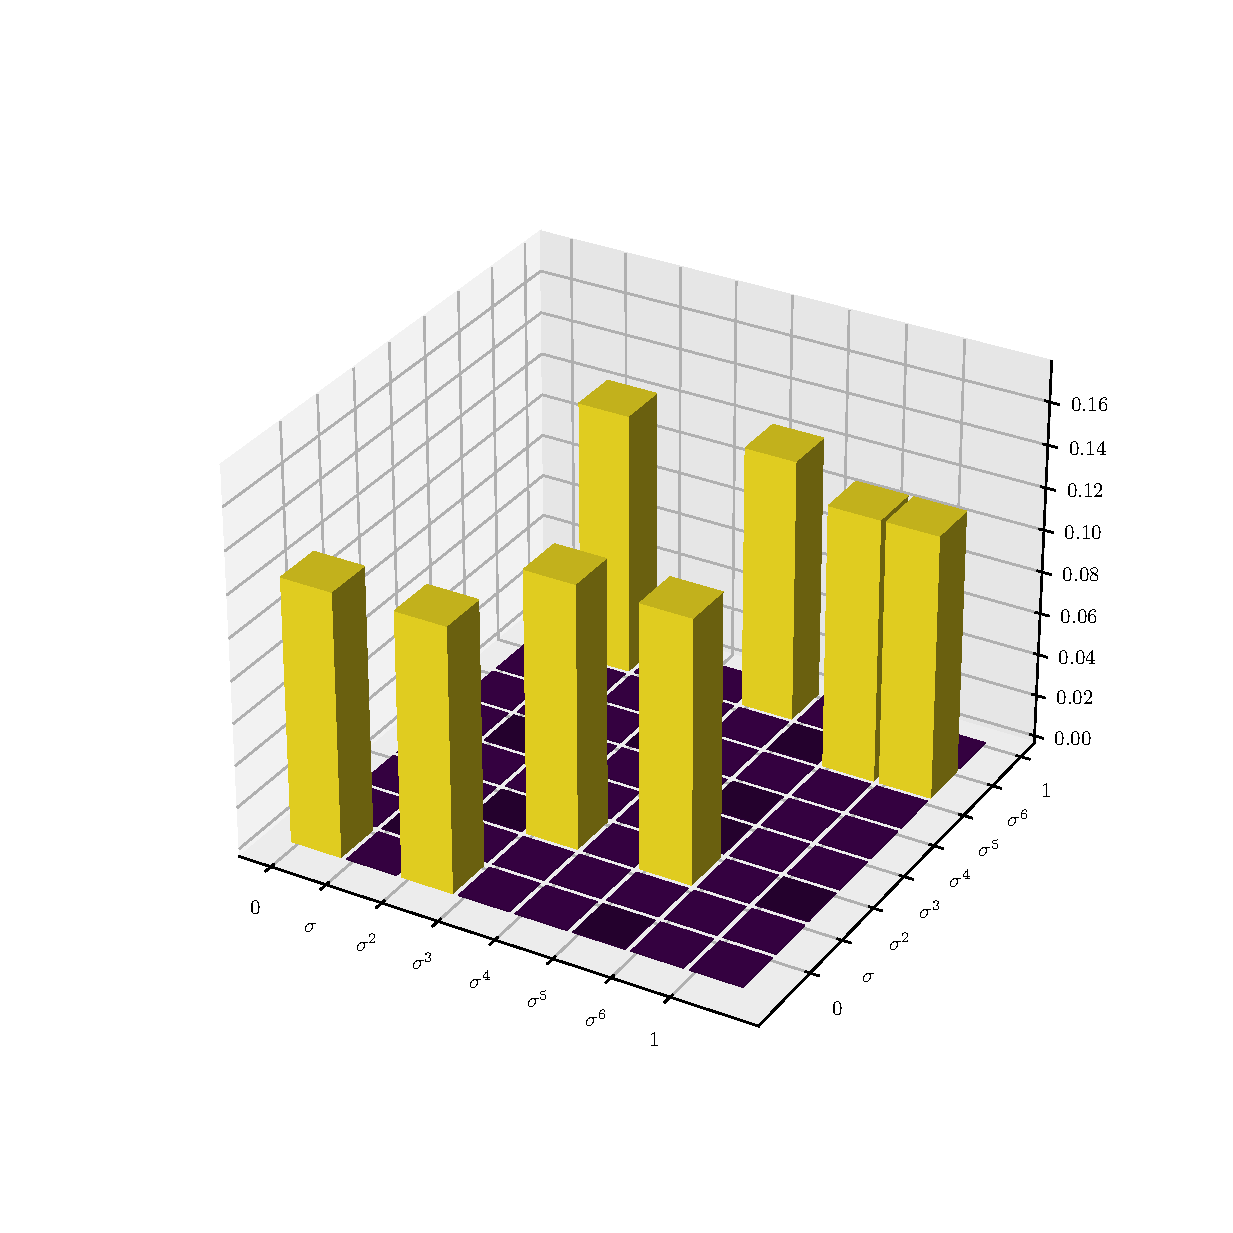
\includegraphics[width=5cm]{abelian_2.eps} }}%
    \qquad
    \subfloat[\centering label
    2]{{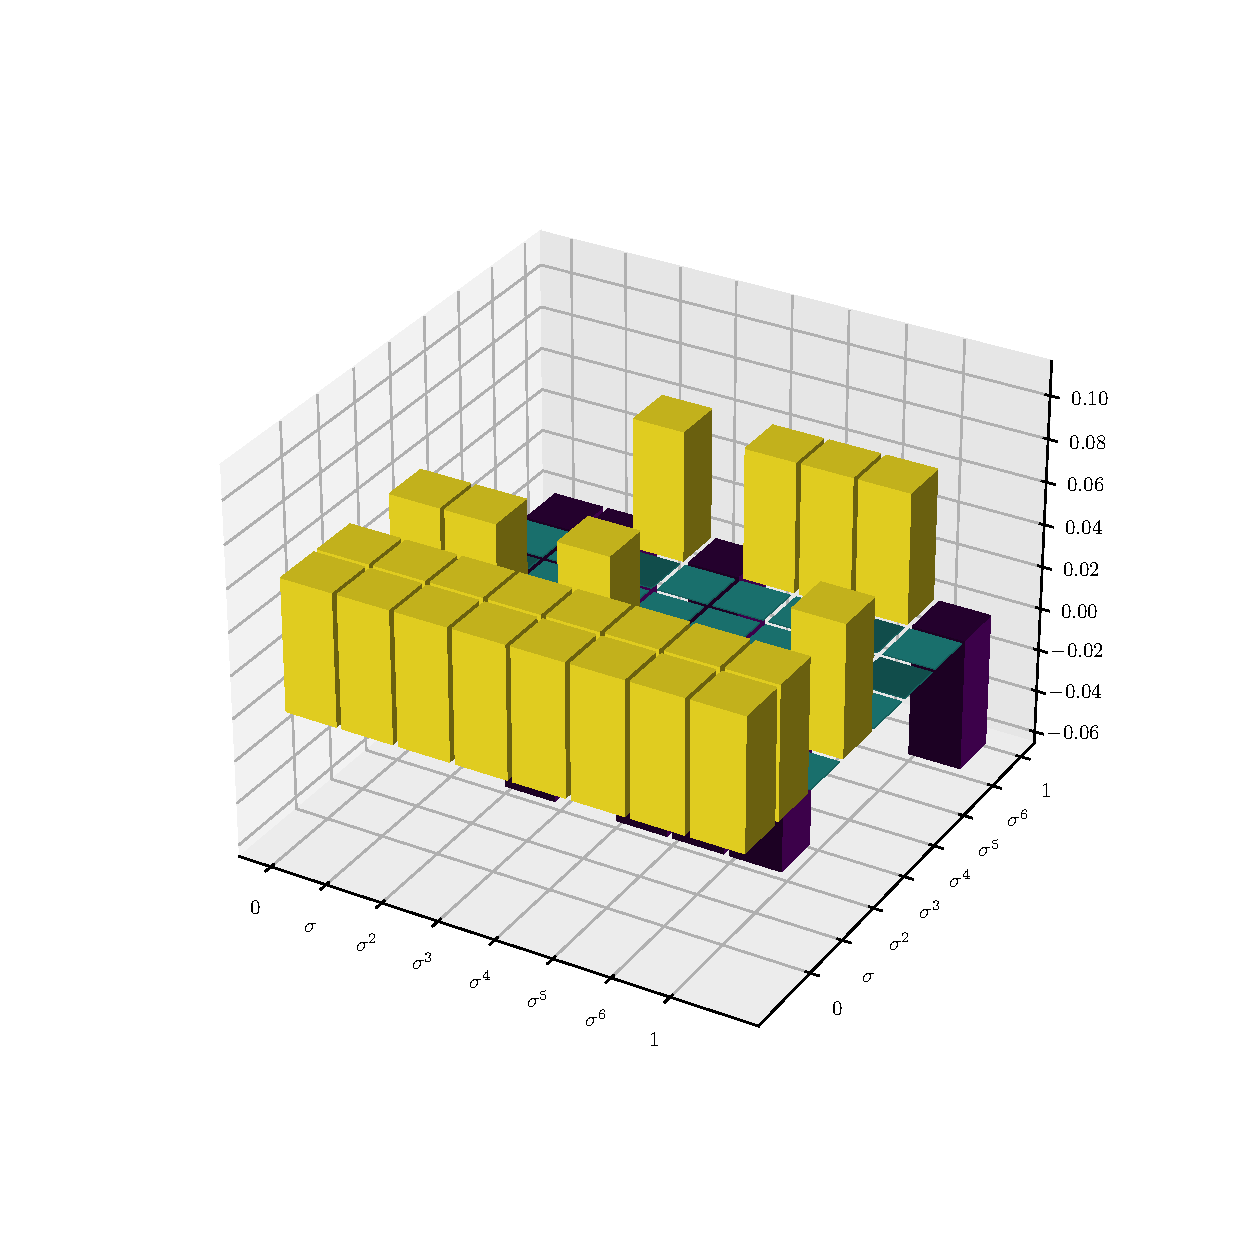
\includegraphics[width=5cm]{non_abelian_40_111.eps} }}%
    \caption{2 Figures side by side}%
    \label{fig1}%
\end{figure}

However, the abovementioned curves \textit{become} abelian for a different
assignment of signs to the phases (\ref{Phib}). For instance, the curve
(\ref{nac}) is abelian by choosing $\Phi_{\alpha,\mu \alpha }(\theta_{k}) =
-\sqrt{\chi\left(\mu \theta_{k}^{2}\right)}$ for any $\mu \neq 0$. Under this
assignment, the following regular curves (\ref{rc}) are abelian:
\begin{enumerate}
  \item if $\phi = \sigma, \sigma^{2}, \sigma^{4}$, then $\phi_{0} = \phi +
    \phi^{2}$;
  \item if $\phi = \sigma^{3}, \sigma^{5}, \sigma^{6}$, then $\phi_{0} = \phi +
    \phi^{2}$;
  \item if $\phi = 1$, $\phi_{0} = 0$.
\end{enumerate}
The curve (\ref{nac1}) is abelian under an assignment where the signs of
$\Phi_{\alpha,\mu \alpha}(\theta_{k})$ depend of the value of the slope $\mu$.

In general, in the three-qubit case and the specific $(3,0,6)$ DPS partition,
certain choices of phase signs $\Phi_{\alpha,\mu \alpha}(\theta_{k})$ can make
all possible commutative curves abelian. The inverse statement is however not
true: for a given curve, it is not always possible to establish a choice of
signs of $\Phi_{\alpha,\beta }(\theta_{k})$ so that this curve becomes abelian
for fixed phases $\Phi_{\alpha,\mu \alpha}(\tau)$.

\section{Conclusions}

The Wigner mapping kernel can be constructed as a sum of projectors into
elements of a complete set of MUBs, which are eignestates of disjoint
stabilizers corresponding to a given partition of the discrete phase-space
into non-intersecting commutative curves. Different partitions lead to
different factorization properties of MUBs, which are required for the
mapping. For qudit systems with odd local dimensions, the Wigner kernel is
factorized in the same form for all possible partitions. This results in
tomographic universality, reflected in the delta-function form of Wigner
functions of any stabilizer state corresponding to any partition.

However, in the case of $n$-qubit systems, the mapping kernel is not
factorizable, and its form depends on the chosen discrete phase-space
partition \cite{Bjork2007}, and on the selected set of stabilizer states in
this core partition, particularly on their phases. Consequently, the qubit
Discrete Wigner Function is not tomographically universal for an arbitrary
election of phases of the stabilizer states used for the Wigner map
construction. Nonetheless, this property is not completely lost. It results
that for a given partition of the DPS there are stabilizer states,
corresponding to commutative curves which do not participate in the
construction of the mapping kernel, such that their DWF are delta-functions.
This means that the probability of detecting these states by measuring in an
arbitrary state is obtained by summing the DWF along the corresponding curve.
This property is directly related to the feasibility of classical simulation of
Pauli observables measurements in such $n$-qubit states (see Theorem 2 in
\cite{Raus17}). However, since the measurement procedure is codified in the
partition of the DPS, only some specific stabilizer states, beyond those used
in the measurement scheme, are classically simulable in a given experimental
setup (for a fixed DPS partition). In other words, different experimental
configurations may lead to different classical simulability outcomes for
stabilizer states. This highlights the role of experimental design and setup in
determining the classical or quantum nature of measurement outcomes. On the
other hand, it is always possible to adjust a detection scheme so that the
Pauli measurements in any particular stabilizer state can be described by a
non-contextual hidden variable model. This supports previously discussed
results \cite{Raus17,contextMagic} that the stabilizer states cannot be
considered as a resource for quantum computation \cite{gottKnill}.

Although we have analyzed only a three-qubit system, the present approach is
extendable to a higher number of qubits. In particular, one can expect that
for any given partition, there are sign assignments such that the DWF of an
arbitrary stabilizer state acquires a delta-function form, i.e. confirms the
tomographic universality of $n$-qubit DWFs under the freedom of the phase
choice. This conjecture has been verified by extensive numerical simulations
and, it can be justified by the same functional form of the recurrence
equation (\ref{phase 2}) for the phase (\ref{Phi}) of any abelian curve.

\appendix

\section{Commutative curves}

In this Appendix we recall some basic properties of commutative curves in
even local dimensions.

Commuting sets constituted by $2^{n}$ different monomials (stabilizers) $\{
\hat{Z}_{\alpha _{\lambda }(\tau )}\hat{X}_{\beta _{\lambda }(\tau )}, \, \tau
\in \mathbb{F}_{2^{n}}\}$ are labelled by points of a discrete grid belonging to
a non-singular curve (i.e., with no self-intersection) $\Gamma^{\lambda }$ that
passes through the origin, $(\alpha (0),\beta (0))=(0,0)\in \Gamma^{\lambda }$
and satisfies

\begin{equation*}
  \tr\left(
    \alpha_{\lambda}(\tau^{\prime})\beta_{\lambda}(\tau)
  \right)
  = \tr\left(
    \alpha_{\lambda}(\tau)\beta_{\lambda}(\tau^{\prime })
  \right),
  \quad \left(
    \alpha_{\lambda }(\tau), \beta_{\lambda}(\tau)
  \right) \in \Gamma^{\lambda}. 
\end{equation*}

A general parametric form of such a curve is given by

\begin{equation}
  \alpha (\tau)
  = \sum_{k=0}^{n-1}\alpha_{k}\,\tau^{2^{k}},
  \quad
  \beta(\tau)
  = \sum_{k=0}^{n-1}\beta_{k} \, \tau^{2^{k}},
  \quad \alpha_{k},\beta_{k}\in \mathbb{F}_{2^{n}},
  \label{curve1a}
\end{equation}

where the coefficients $\alpha_k$ and $\beta_k$ are such that $\sum_{m \neq k}
\tr(\alpha_{m}\beta_{k})=0$, which implies

\begin{equation}
  \lbrack
  \hat{Z}_{\alpha (\tau )}\hat{X}_{\beta (\tau )},
  \hat{Z}_{\alpha (\tau^{\prime })}\hat{X}_{\beta(\tau^{\prime})}
  ] = 0 \, , \;\; \left(
    \alpha_{\lambda}(\tau),\beta_{\lambda}(\tau)
  \right) \in \Gamma ^{\lambda }.
  \label{stab}
\end{equation}

It is worth noting that $n$ appropriately chosen points of the curve, e.g. $\tau
= \{\theta _{1},\ldots,\theta_{n}\}$ generate the entire curve. This is because
the set of points of these curves form an abelian group where each element is of
order two, and therefore is isomorphic to $\mathbb Z_{2}^n$.

The regular curves, which are non-degenerated in at least one of the directions
$\alpha$ or $\beta$ (i.e., they take on all the values of the field in such a
direction), can be represented in the explicit form,

\begin{equation}
  \beta = f(\alpha) = \sum_{k=0}^{n-1} \phi_{k} \, \alpha^{2^{k}}
  \quad \text{or}
  \quad \alpha = g(\beta) = \sum_{k=0}^{n-1} \psi_{k}\,\beta^{2^{k}},
  \label{RC}
\end{equation}

where $\phi_{k},\psi_{k} \in \mathbb{F}_{2^{n}}$ satisfy the following
commutativity restrictions,

\begin{equation}
  \phi_{k}
  = \phi _{n-k}^{2^{k}}\,, \qquad \psi_{k}
  = \psi_{n-k}^{2^{k}}\,, \qquad k=1,\ldots,
  \left\lfloor \frac{n-1}{2}\right\rfloor,
  \label{Acc}
\end{equation}

where $\left\lfloor . \right\rfloor$ denotes the integer part and in particular
for even $n$ the additional restriction:
\begin{equation}
  \phi_{n/2}
  = \phi_{n/2}^{2^{n/2}}, \qquad \psi_{n/2}
  = \psi_{n/2}^{2^{n/2}}.
\end{equation}

The degenerate (or exceptional) curves are characterized by multiple appearances
of the admissible points in both directions $\alpha $ and $\beta$. In other
words, for every point $(\alpha_{j},\beta_{j})$ of such a curve, $\alpha_{j}$ and
$\beta_{j}$ take on only $2^{n-r_{\beta }}$ and $2^{n-r_{\alpha}}$ different
values respectively, where $r_{\alpha }$ and $r_{\beta }$ are the degrees of
degenerations along the corresponding axes. The admissible points of such curves
are fixed by the relations $\tr(\sigma_{j}\beta)=0$ and
$\tr(\sigma_{k}\alpha)=0$ where $\sigma_{j}, \sigma_{k}$ are some given elements
of $\mathbb{F}_{2^{n}}$.

The partitions of the DPS constituted by $2^{n}+1$ commutative curves are
classified by their factorization structures (\ref{curve_part}), $\lambda
=\{m_{1},m_{2},\ldots ,m_{n}\}\,$, where $\sum_{k}$ $m_{k}=2^{n}+1$, which
indicates the number and the lengths of the commuting sub-blocks of the
stabilizers labelled by the points of a curve. Locally equivalent stabilizers
can be labelled by points of different curves, but  have the same factorization
structure. On the other hand, curves with different factorization structures are
not locally equivalent.

In particular, in the partition given by Eq. (\ref{rays}) there are three
completely factorized rays ($\beta = 0, \alpha = 0$, and $\beta = \alpha$),
i.e., of the structure $\{1,1,1\}$, and the other six rays have the structure
$\{3\}$, so that the whole partition is $(3,0,6)$.

The $(0,9,0)$ partitions include only curves with the factorization $\{1,2\}$,
and always contain exceptional curves. One example of those partitions is given
by the following seven regular and two exceptional curves:

\begin{enumerate}[a)]
  \item Regular curves
    \begin{equation}
      \begin{array}{ll}
        \alpha = \sigma^{2}\beta + \sigma^{3}\beta^{2} + \sigma^{5}\beta^{4},
        \qquad
        & \alpha = \sigma^{6}\beta + \sigma^{3}\beta^{2} +
        \sigma^{5}\beta^{4},\\[4pt]
        \beta = \sigma^{2}\alpha + \sigma^{3}\alpha^{2} + \sigma^{5}\alpha^{4},
        \qquad
        & \beta = \sigma^{6}\alpha^{2} + \sigma^{3}\alpha^{4}, \\[4pt]
        \alpha = \beta + \sigma^{6}\beta^{2} + \sigma^{3}\beta^{4},
        \qquad
        & \beta = \alpha + \sigma^{3}\alpha^{2} + \sigma^{5}\alpha^{4}, \\[4pt]
        \alpha = \sigma^{3}\beta^{2} + \sigma^{5}\beta^{4},
        \qquad
        &
      \end{array}
    \end{equation}

  \item Exceptional curves
    \begin{eqnarray}
      \beta^{2} + \sigma^{5}\beta
      &=& \sigma^{2}\alpha^{2} + \sigma^{6}\alpha,
      \qquad 
      \tr(\sigma^{4}\beta)=0,
      \quad
      \tr(\sigma^{5}\alpha)=0;
      \nonumber \\
      && \\
      \beta^{2} + \sigma^{2}\beta
      &=& \sigma^{6}\alpha^{2} + \sigma^{5}\alpha,
      \qquad
      \tr(\sigma^{6}\beta)=0,
      \quad
      \tr(\sigma^{2}\alpha)=0.
      \nonumber
    \end{eqnarray}
\end{enumerate}

\begin{thebibliography}{99}
\bibitem{wigner} Wigner, E. On the quantum correction for thermodynamic
equilibrium. \textit{Phys. Rev. A} \textbf{1932}, \textit{40}, 749-759
[doi:10.1103/PhysRev.40.749].

\bibitem{bloch} Bloch, F. Zur Theorie des Austauschproblems und der
Remanenzerscheinung der Ferromagnetika. \textit{Zeits F. Physik} \textbf{1932%
}, \textit{74}, 295-335 [doi:10.1007/978-3-662-41138-4].

\bibitem{groenewold} Groenewold, H. J. On the principles of elementary
quantum mechanics. \textit{Physica} \textbf{1949}, \textit{12}, 405-460.
[doi:10.1016/S0031-8914(46)80059-4].

\bibitem{moyal} Moyal, J. E. Quantum mechanics as a statistical theory. 
\textit{Mathematical Proceedings of the Cambridge Philosophical Society} 
\textbf{1947}, \textit{45}, 99-124. [doi:10.1017/S0305004100000487].

\bibitem{qoptics} Mandel, L.; Wolf, E. Coherence Properties of Optical
Fields. \textit{Rev. Mod. Phys.} \textbf{1965}, \textit{37}, 231-287.
[doi:10.1103/RevModPhys.37.231]

\bibitem{electron1} Barker, J. R.; Murray, S. A quasi-classical formulation
of the Wigner function approach to quantum ballistic transport. \textit{%
Phys. Lett. A} \textbf{1983}, \textit{93}, 271-274.
[doi:10.1016/0375-9601(83)90786-7].

\bibitem{electron2} Lin, J.; Chiu, L. C. Quantum theory of electron
transport in the Wigner formalism. \textit{J. Appl. Phys.} \textbf{1985}, 
\textit{57}, 1373-1376. [10.1063/1.334489].

\bibitem{berry} Berry, M. V. Semi-classical mechanics in phase space: A
study of Wigner's function. \textit{Philos. Trans. R. Soc. A} \textbf{1977}, 
\textit{287}, 237-271. [doi:10.1098/rsta.1977.0145]

\bibitem{spin1} O'Connell R. F.; Wigner E. P. Manifestations of Bose and
Fermi statistics on the quantum distribution functionfor systems of spin-0
and spin- 1/2 particles. \textit{Phys. Rev. A} textbf{1984}, \textit{30},
2613-2618. [doi:10.1103/PhysRevA.30.2613].

\bibitem{spin2} Cohen, M.; Scully, M. O. Joint Wigner distribution for
spin-1/2 particles. \textit{Foud. Phys.} \textbf{1986}, \textit{16},
295-310. [doi:10.1007/BF01882690].

\bibitem{wootters1} Wootters, W. K. A Wigner-function formulation of
finite-state quantum mechanics. \textit{Annals Phys.} \textbf{1987}, \textit{%
176}, 1-21. [doi:10.1016/0003-4916(87)90176-X].

\bibitem{gibbons} Gibbons, K. S.; Hoffman, M. J.; Wootters, W. K. Discrete
phase space based on finite fields. \textit{Phys. Rev. A} \textbf{2004}, 
\textit{70}, 062101. [doi:10.1103/PhysRevA.70.062101].

\bibitem{gottKnill} Gottesman, D. The Heisenberg representation of quantum
computers. In \textit{Group 22: International Colloquium on Group
Theoretical Methods in Physics}, Proceedings of 22nd International
Colloquium, Group22, ICGTMP'98, Hobart, Australia, July 13-17, 1998; S. P.
Corney, R. Delbourgo, P. D. Jarvis, Eds.; International Press: Cambridge,
MA, 1999, pp. 32-43. [doi:]

\bibitem{galvao} Galv\~ao, E.F. Discrete Wigner functions and quantum
computational speedup. \textit{Phys. Rev. A} \textbf{2005}, \textit{71},
042302. [doi:10.1103/PhysRevA.71.042302].

\bibitem{cormick} Cormick, C.; \textit{et al.} Classicality in discrete
Wigner functions. \textit{Phys. Rev. A} \textbf{2006}, \textit{73}, 012301.
[doi:10.1103/PhysRevA.73.012301]

\bibitem{gross} Gross, D. Hudson's theorem for
finite-dimensional quantum systems. \textit{J. Math. Phys. A} \textbf{2006}, 
\textit{47}, 122107. [doi:10.1063/1.2393152]

\bibitem{WignerNegResource} Veitch, V. C.; Ferrie, C.; Gross, D.; Emerson,
J. Negative quasi-probability as a resource for quantum computation. \textit{New
J. Phys.} \textbf{2012}, \textit{14}, 113011.
[doi:10.1088/1367-2630/14/11/113011]

\bibitem{Raus17} Raussendorf, R.; Browne, D.E.; Delfosse, N.; Okay, C.;
Bermejo-Vega, J. Contextuality and Wigner-function negativity in qubit
quantum computation. \textit{Phys. Rev. A} \textbf{2017}, \textit{95}
052334. ][doi:10.1103/PhysRevA.95.052334]

\bibitem{UniqueWF} Schmid, D.; Du, H.; Shelby, J. H.; Pusey, M. F.
Uniqueness of Noncontextual Models for Stabilizer Subtheories. \textit{Phys.
Rev. Lett.} \textbf{2022}, \textit{129}, 120403.
[doi:10.1103/PhysRevLett.129.120403]

\bibitem{cohomo} Raussendorf, R.; Okay, C.; Zurel, M.; Feldmann, P. The role
of cohomology in quantum computation with magic states. \textit{Quantum} 
\textbf{2023}, \textit{7}, 979. [doi:10.22331/q-2023-04-13-979].

\bibitem{Saniga2004} Saniga, M.;Planat, M.; Rosu, H. Mutually unbiased bases
and finite projective planes. \textit{\ J. Opt. B: Quantum Semiclass. Opt.} 
\textbf{2004}, \textit{6} L19-L20. [doi:10.1088/1464-4266/6/9/L01]

\bibitem{ivanovic} Ivanovic, I. D. Geometrical description of quantal state
determination. \textit{J. Phys. A.} \textbf{1984}, \textbf{14}, 3241-3245.
[doi:10.1088/0305-4470/14/12/019]

\bibitem{mubs1} Wootters, W. K.; Fields, B. D. Optimal State-Determination
by Mutually Unbiased Measurements. \textit{Ann. Phys.} \textbf{1989}, 
\textit{191} 363-381. [doi:10.1016/0003-4916(89)90322-9]

\bibitem{mubs2} Klappenecker, A.; R{\"{o}}tteler, M. Constructions of
mutually unbiased bases. In \textit{Lecture Notes in Computer Science Vol.
2948: Finite Fields and Applications}, Procceedings of 7th International
Conference, Fq7, Toulouse, France, May 5-9, 2003; G.~Mullen, A.~Poli,
H.~Stichtenoth, Eds. Springer: Germany, Berlin, 2003, pp. 137--144.

\bibitem{Bandyopadhyay2002} Bandyopadhyay, S.; Boykin, P.~O.;Roychowdhury,
V.; Vatan, F. A new proof for the existence of mutually unbiased bases. 
\textit{Algorithmica} \textbf{2002}, \textit{34}, 512--528.
[doi:10.1007/s00453-002-0980-7]

\bibitem{GS2} Klimov, A. B.; Romero, J. L.; Bj\"{o}rk, G.; S\'{a}nchez-Soto,
L. L. Discrete phase-space structure of n-qubit mutually unbiased bases. 
\textit{Ann.Phys.} \textbf{2009}, \textit{324}, 53-72.
[doi:10.1016/j.aop.2008.10.003]

\bibitem{JPA09} Klimov, A. B.; Romero, J. L.; Bj{\"{o}}rk, G.; S{\'{a}}%
nchez-Soto, L. L. Geometrical approach to mutually unbiased bases. \textit{%
J. Phys. A: Math. Gen.} \textbf{2007}, \textit{40}, 9177.
[doi:10.1088/1751-8113/40/14/014]

\bibitem{Bjork2007} Pittenger, A.~O.; Rubin, M.~H. Wigner functions and
separability for finite systems. \textit{J. Phys. A: Math. Gen.} \textbf{2005%
}, \textit{38} 6005-6036. [doi:10.1088/0305-4470/38/26/012]

\bibitem{DFW11} Wootters, W.K.; A Wigner-function formulation of
finite-state quantum mechanics. \textit{Ann. Phys.} \textbf{1987}, \textit{\
176}, 1-21. [doi:10.1016/0003-4916(87)90176-X]

\bibitem{DFW12} Delfosse, N.; Guerin, P.A.; Bian, J.; Raussendorf, R. Wigner
Function Negativity and Contextuality in Quantum Computation on Rebits. 
\textit{Phys.Rev. X} \textbf{\ 2105 }, \textit{5}, 021003.
[doi:10.1016/0003-4916(87)90176-X]

\bibitem{contextMagic} Howard, M.; Wallman, J.; Vietch, V.; Emerson, J.
Contextuality supplies the `magic' for quantum computation. \textit{Nature}
\textbf{214}, \textit{510}, 351-355.  [doi:10.1038/nature13460]

\bibitem{WignerContext} Delfosse, N. \textit{et al.} Equivalence between
contextuality and negativity of the Wigner function for qudits. \textit{New
J. Phys.} \textbf{2017}, \textit{19}, 123024. [doi:10.1088/1367-2630/aa8fe3]

\bibitem{qip17} Mu\~noz, C.; Klimov, A. B.; Sanchez-Soto, L. L. Discrete
phase-space structures and Wigner functions for $N$ qubits. \textit{Quantum
Inf. Process} \textbf{2017}, \textit{16}, 158. [doi:10.1007/s11128-017-1607-x]

\bibitem{FF} Lidl, R.; Niederreiter, H. \textit{Introduction to Finite
Fields and their Applications}, 2nd ed.; Cambridge University Press,
Cambridge, United Kingdom, 1994.

\bibitem{Schwinger1} Schwinger, J. UNITARY OPERATOR BASES. \textit{Proc.
Natl. Acad. Sci. USA} \textbf{1960}, \textit{46}, 570.
[doi:10.1073/pnas.46.4.570]

\bibitem{Schwinger2} Schwinger, J. UNITARY TRANSFORMATIONS AND THE ACTION
PRINCIPLE. \textit{Proc. Natl. Acad. Sci. USA} \textbf{1960}, \textit{46},
883. [doi:10.1073/pnas.46.6.883]

\bibitem{factor1} Lawrence, J.; Brukner, \v{C}.; Zeilinger, A. Mutually
unbiased binary observable sets on $N$ qubits. \textit{Phys. Rev. A} \textbf{%
2002}, \textit{65}, 032320. [doi:10.1103/PhysRevA.65.032320]

\bibitem{factor2} Romero, J. L.; Bj\"{o}rk, G.; Klimov, A. B.; S\'{a}%
nchez-Soto, L. L. Structure of the sets of mutually unbiased bases for $N$
qubits. \textit{Phys. Rev. A} \textbf{2005}, \textit{72}, 062310.
[doi:10.1103/PhysRevA.72.062310]

\bibitem{Durt2006} Durt, T. About Weyl and Wigner tomography in
finite-dimensional Hilbert spaces. \textit{Open Sys. Inf. Dyn.} \textbf{2006}%
, \textit{13}, 403--413. [doi:10.1007/s11080-006-9022-2]

\bibitem{DFW2-1} Vourdas, A. Quantum systems with finite Hilbert space. 
\textit{Rep. Prog. Phys.} \textbf{2004}, \textit{67}, 267.
[doi:10.1088/0034-4885/67/3/R03]

\bibitem{DFW2-2} Vourdas, A. Factorization in finite quantum systems. 
\textit{\ J. Phys. A: Math. Gen.} \textbf{2003}, \textit{36}, 5645.
[doi:10.1088/0305-4470/36/20/319]

\bibitem{DFW2-3} Paz, J.P.; Roncaglia, A. J.; Saraceno, M. Qubits in phase
space: Wigner-function approach to quantum-error correction and the
mean-king problem. \textit{\ Phys. Rev. A} \textbf{2005}, \textit{72},
012309. [doi:10.1103/PhysRevA.72.012309]

\bibitem{DFW2-4} Bjork, G.; Klimov, A. B.; Sanchez-Soto, L.L. The discrete
Wigner function. In \textit{Progress in Optics}, 1st ed.; Wolf, E., Ed.;
Elsevier: Amsterdam, The Netherlands, 2008, Volume 51, pp. 469-516.
[doi:10.1016/S0079-6638(07)51007-3]

\bibitem{klimov06} Klimov, A. B.; Mu\~{n}oz, C.; Romero, J. L. Geometrical
approach to the discrete Wigner function in prime power dimensions. \textit{%
J. Phys. A: Math. Gen.} \textbf{2006}, \textit{39}, 14471.
[doi:10.1088/0305-4470/39/46/016]
\end{thebibliography}

\end{document}
